%!TEX root = ../thesis.tex
%*******************************************************************************
%****************************** Third Chapter **********************************
%*******************************************************************************
\chapter{Event history analysis of an ecological tension zone in Maranhão using satellite imagery}

% **************************** Define Graphics Path **************************
\ifpdf
    \graphicspath{{Chapter3/}}
\else
    \graphicspath{{Chapter3/}}
\fi

\begin{abstract}
Deforestation rates in Brazil had decline in the past decade. Great part of this effort comes from the environmental policies used as instruments to encourage forest preservation. Focusing on the ecological tension zone of Maranhão that separates it in two parts, we estimate the probability of a transition between intact forest to disturbed forest, given the risk factors, and conditional on the time elapsed until the occurrence of the transition. We check if the probability of deforestation was higher in the region not controlled by a specific environmental policy. To this end, we use remote sensing sources to construct a time event dataset at individual pixel level and, we conduct a survival analysis in both regions. The results suggest that forests inside the specific surveillance policy area had a lower probability of survival comparing to the area not covered by the environmental policy. Forested pixels close to protected areas,  which include conservation units and indigenous land, had a higher chance of being cleared comparing to forested pixels far from these special zones. The presence of clouds was an active barrier to the legal compliance and, since the studied area has no systematic differences, we can agree on the lack of effectiveness due to cloud barrier. With our robustness check, it is acceptable that the environmental policy could not detain deforestation during the last two decades in the ecotonic region of Maranhão.

\noindent{\bf Keywords: Remote Sensing, Survival Analysis, Environmental Policies, Deforestation} 

\end{abstract}

\section{Introduction}
\label{S:3.1}
%Describing policies that decreased the rate of deforestation in Brazil
The clear-cutting of forests plays a central role in many environmental threats of our time, including global climate change, habitat degradation, and species extinction. However, deforestation rates in Brazil had decline in the past decade. Great part of this effort comes from the environmental policies used as instruments to encourage forest preservation. The best example is the satellite monitoring program that allowed the environmental police to fastening the response to punish clear-cutting agents.\footnote{In 2004, the Brazilian government created the Action Plan for the Prevention and Control of Deforestation in the Legal Amazon (PPCDAm in Portuguese). Its purpose was to plan development, control land use and ensure compliance with the environmental law and promote sustainable practices. In order to control land use and prevent further deforestation, the PPCDAm also included the satellite-based monitoring programme PRODES (Projeto de Estimativa do Desflorestameno da Amaz\^{o}nia in Portuguese) \citep{inpe} that recorded incidents of deforestation throughout the year within the policy area.} % the establishment of several national parks, national forests, extractivist and biological reserve areas, and the recognition of indigenous and traditional territories \citep{araujo}.

%Border issue 
%\citet{burgess_costa_olken_2018} showed the differences of deforestation rate at the Brazilian international border. According to their results, the differences were higher and significant until 2006 in the Brazilian portion, right after the implementation of the satellite environmental policy. After that period, the differences disappeared. Although the results lead to a significant positive impact from the policy, it is important to understand these differences \textit{within} Brazilian biomes borders since the rates are a constant risk to the environment and to the increasing concerns on climate change.

%Linking Chapter 2 %Cloud issue 
A recent study (see Chapter 2) observed the trends of deforestation in two regions, under different environmental policies, of an ecological tension zone (ecotone forest) in Maranhão.\footnote{Ecotone is defined as the transition area between two or more distinct habitats or ecosystems, which may have characteristics of both or their own. Secondary Vegetation includes the various stages of natural succession in areas where there was human intervention for land use, whether for mining, agricultural or livestock purposes, or discharging the primary vegetation \citep{SANTOS-FILHO_2013}.} For the environmentally regulated region, deforestation process shifted from dry season to raining season. Besides that, the study indicated that part of deforestation displaced to the region not controlled by the environmental policy. Apparently, the policy faded in areas of biome transition that coincided with the delimitation of the surveillance policy. In addition, behaviour changes might have emphasised this problem. Event history analysis could confirm these findings by considering the heterogeneity within the region because not all sites within ecological tension zone have the same risk of deforestation. 

%\citet{Vina_2004} investigated the rates and patterns of land-cover change along a portion of the Colombia-Ecuador border during a 23-yr period using satellite data to document the rates. Satellite change detection analysis showed that the annual rates of deforestation were considerably higher for the Colombian side of the border. \citet{Chicas_2017}  studied the trans-boundary deforestation history and patterns in protected areas along the Belize-Guatemala border and indicated that failure to integrate buffer communities, coordinate among managing organisations and establish strong bi-national collaboration has resulted in continued ecological and environmental degradation. 

%Existing Related Literature of Survival Analysis and Deforestation in Borders - Not found. :(
%\citet{Egler_2013} conducted a study in an extensive rain forest-savanna ecotone, located in the south border of Amazon biome showed a significant reduction in production and commercialisation of extractive products in the region. In his work, land use, socioeconomic and conservation indicators, combined with statistical analysis, were used to understand forces associated with patterns of deforestation. The author revealed that the main conservation policy in Mato Grosso was the creation of protected areas. 
\citet{vance_2002} estimated a spatially explicit model of forest clearance process in the southern Mexico implementing a time event analysis to identify the effect of households on the probability of deforestation. The results showed a non-linear probability of forest clearance. \citet{greenberg_2005} assessed the impact of spatial, cultural and economic factors on deforestation using survival analysis on satellite data from eastern Ecuador. Their results showed that deforestation prediction was higher when there was a proximity  to roads. Until now, studies combining satellite data in areas of ecotone forest to detect time event (survival) analysis of the risk of deforestation process remains scarce in the Brazilian literature.\footnote{Monitoring the transitional biome is difficult due to the high heterogeneity of the forests (open and dense forest, for example) which are substantially influenced by the climatic seasonality \citep{bayma_sano_2015}. Also, there is no environmental policy in place to prevent rampant deforestation. However, in the context of the Amazon region which is under an specific environmental policy, it is arguably crucial to understand the dynamic of the transitional forest borders and its potential to influence adjacent Amazon forests since it provides a valuable endpoint from which climate and anthropogenic related aspects in the Amazon forest my be better understood.} In this sense, it is conceivably that this is one of the contributions of this study.

Our study, then, focuses on the ecological tension zone of Maranhão because is divided by an artificial line that separates it in two parts: the Legal Amazon Maranhão and the Cerrado Maranhão. This division, occurring approximately 44$^{\circ}$ west of the meridian, allows the state to be divided in terms of environmental policies. This scenario provides a unique natural experiment of deforestation in the Legal Amazon Maranhão and Cerrado Maranhão since the former has been subject to fundamentally different environmental policies compared to the latter. The crossed area is homogeneous in several aspects such as biota, institutions, and, climate with the only difference being the surveillance environmental program that is observed in only one part of the region.

We use this spatial division to estimate the probability of a transition between intact forest to disturbed forest, given the risk factors, and conditional on the time elapsed until the occurrence of the transition. We were interested in addressing (1) if the probability of deforestation was higher in the region not controlled by a specific environmental policy, (2) what factors may be influencing the risk of the two regions to be deforested? And, (3) if changing behaviour undermined the effect of the policy.

To this end, we use remote sensing sources (MODIS Vegetation Indices (MOD13Q1) product) to construct a time event dataset at individual pixel level. The risk factor or covariates variables were acquired in shapefile format from different sources at the same level. Using this method, it is possible to predict the probability of deforestation and determine which covariates affect the risk of forest clearing at small-scale level. Holding this information, conservation methods can be better formulated and environmental policies can be better improved for the Maranhão state.

According to the survival analysis results, the forests inside the specific surveillance policy area had a lower probability of survival comparing to the area not covered by the environmental policy. Forested pixels close to protected areas,  which include conservation units and indigenous land, had a higher chance of being cleared comparing to forested pixels far from these special zones. The presence of clouds was an active barrier to the legal compliance and, since the studied area has no systematic differences, we can agree on the lack of effectiveness due to cloud barrier. With our robustness check, it is acceptable that the environmental policy could not detain deforestation during the last two decades in the ecotonic region of Maranhão.


\section{Material and Methods}
\label{S:2}

%Colocar o contexto do estudo, acho que puxando o link do capitulo 2?!

\subsection{Study Context} %mudar o titutlo

%Falar das caracteristicas da regiao estudada

In the central part of Maranhão there is a contact area between the Amazonian and Cerrado biomes, where it is possible to observe a mosaic of savanna vegetation \textit{Cerrado} and open and dense forest formation which configures as an Ecological Tension Zone (ETZ). Authors discuss the difficulty of delimiting forest areas in transitional and / or ecological tension regions, mainly Cerrado - Amazon Forest due to the innumerable indentations and interpenetration of savanna formations in the territory of the Legal Amazon. Areas with these characteristics can be found in the states of Amazonas, Mato Grosso, Pará, Tocantins and, specially, in Maranhão. \citet{GARCIA201716} studied part of the Maranhão central region and defined forest as a combination of riparian forest, transitional forest, and Cerrado woodland which definition is adopted in this study.

In Maranhão, much of deforestation is linked to economic development. The economic growth resulted in growing demand for agricultural and forest derived products, like soy, timber and beef. The main causes of deforestation are assumed to be acting aggregated and the government finds these causes are the easiest and the most accessible ways of responding to their increasing economic pressures \citep{GEIST,CULAS11,CELENTANO_2017}. 


%Falar que nao ha uma estatistica oficial para municipios na parte do MA mas nao para o ML

Previous studies focused on the effectiveness of the environmental policy in the Amazon tropical forests and observed that through specific environmental policies, such as PRODES/DETER, it had a positive impact on curbing deforestation in that region \citep{nepstad2_2014, NEPSTAD, RICHARDS, RICHARDS2, CELENTANO_2017}. Since Cerrado Maranhão's is not under the same policy, the incentives to curb deforestation are rare and research is in need of official dataset that is continuous and at a desegregated level to tackle local deforestation processes.\footnote{Importantly, in July 2018, the National Institute of Spatial Research (INPE in Portuguese) together with several other institutions published a dataset covering annual and biannual of Cerrado biome deforestation at state and national level. From the dataset, it is shown that deforestation in great Cerrado Maranhão, which includes the transitional forest, has been two times higher than in the Amazon region of Maranhão.}\footnote{In order to control for degradation of the forest by selective logging and forest fires, the government uses the DETER program. In addition, two other systems were introduced in 2007: DEGRAD (Mapeamento da Degradaç\~{a}o Florestal na Amaz\^{o}nia Brasileira in Portuguese), for mapping forest degradation in the Legal Amazon, and DETEX (Mapeamento da Cobertura Florestal na Amaz\^{o}nia Brasileira in Portuguese), for detecting logging operations in the Legal Amazon region \citep{VALERIANO}. In order to control land use and prevent further deforestation, the PPCDAm  also includes the satellite-based monitoring programme PRODES (Projeto de Estimativa do Desflorestameno da Amaz\^{o}nia in Portuguese) \citep{inpe} that attempts to record incidents of deforestation throughout the year within the policy area. All the data gathered by the action plan are used to enforce the PPPCDAm plan, which includes the issuing of fines for agents who clear or damage the forest, embargoes of areas in the process of being cleared with the confiscation of equipment, and restrictions on access to subsidised credit \citep{AUBERTIN}.} 

%Colocar a partir daqui que no capitulo anterior se viu que os trends sao diferents quando olhando as duas regions por season. e que eh necessario saber se alem de ter dado o shift, a policy se mostrou efetiva quando compararada com regioes fora da LM.

A previous study of deforestation trends (see Chapter 2) showed that there is evidence of human behaviour changes due to the environmental monitoring policy and that cloud cover may have acted as an impediment to the performance of that environmental program. In turn, this study proposes to investigate whether the environmental policy was effective in that region. We were interested in addressing (1) if the probability of deforestation was higher in the region not controlled by a specific environmental policy, (2) what factors may be influencing the risk of the two regions to be deforested? and, (3) whether changing behaviour undermined the effect of the policy. More specifically, we want to examine if the policy was sufficient and capable of increasing or maintained the probability of forest remaining since the rate of deforestation decreased in the last fifteen years (see fig \ref{fig:defAmazonMA}). To explore this assumption, we study the Ecological Tension Zone of Maranhão.

\begin{figure}[H]
  \centering
  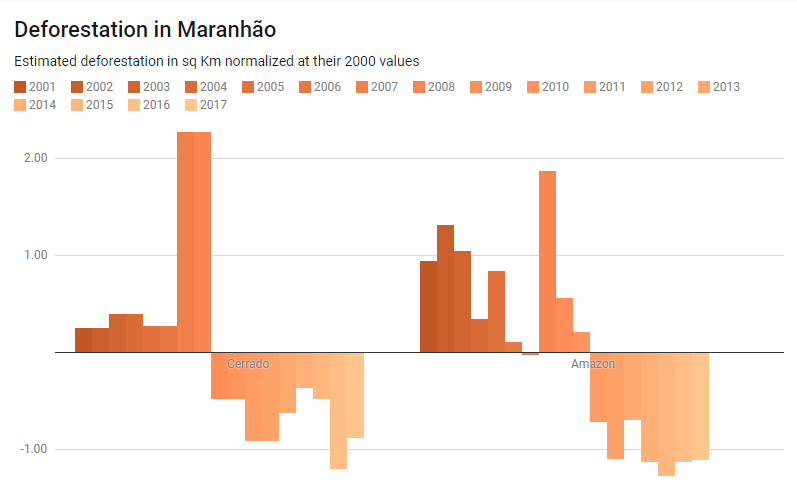
\includegraphics[width=1\textwidth, inner]{Normalizeddeforestation.png}
\caption{Source: \citep{MMMAwebsite}.}
\label{fig:defAmazonMA}
\end{figure}

%Falar sobre a area que o estudo abrange, em termos dos municipios. Que munics sao esses?
\subsubsection{Site}
The studied area comprises a total of 29,307 km$^{2}$ and corresponds to 21 municipalities. All the municipalities are crossed by the artificial division that occurs approximately 44$^{\circ}$ west of the meridian and was established in 1953 in order to plan the economic development of the region comprised of the tropical forest areas of Maranhão state called Legal Maranhão (LM). We depict this delineation in Figure \ref{fig:delimitacao}.

\begin{figure}[H]
  \centering
  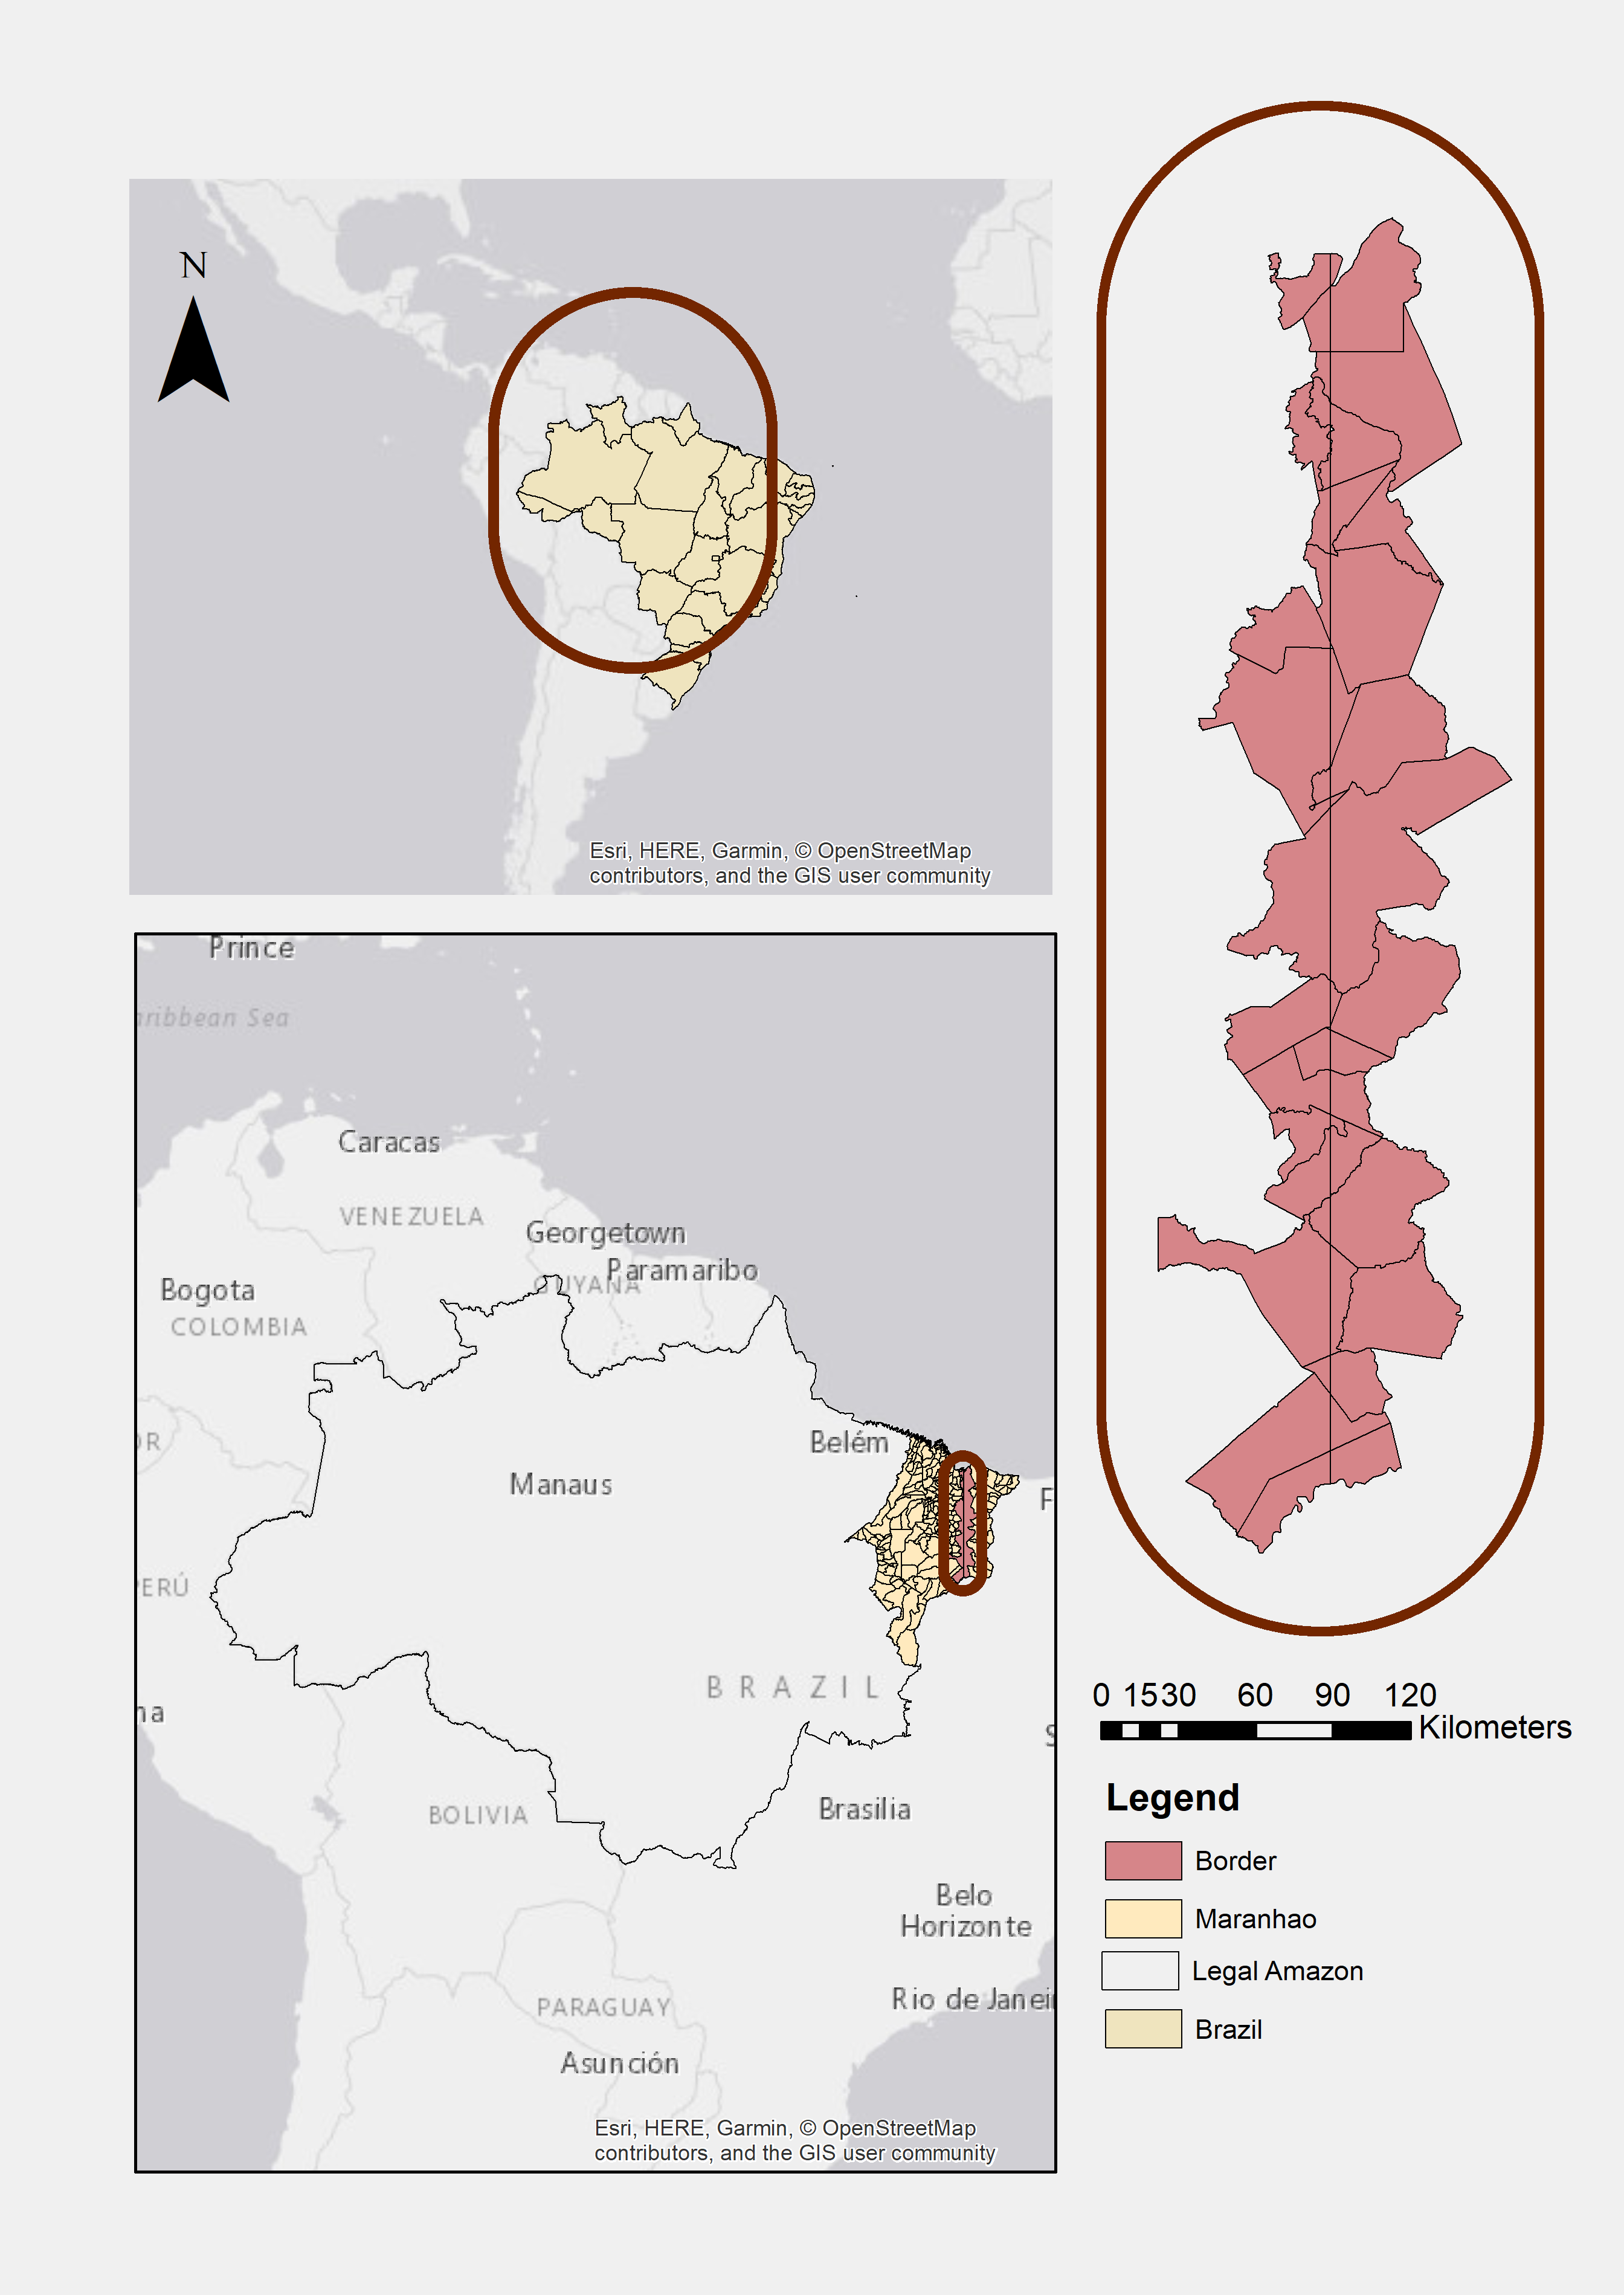
\includegraphics[width=1\textwidth, inner]{Chapter3/MaranhaoChapter3_Fig1.png}
\caption[Map of Maranhao Studied Area]{Map of Maranhao Studied Area. The vertical line in the Border refers to the artificial line that divides Legal Maranhao and Cerrado Maranhao. Source: \citep{MMMAwebsite,nugeo_2018}.}
\label{fig:delimitacao}
\end{figure}

According to \citet{ferreira_2008, CELENTANO_2017, costa_2018}, recent forest losses in the studied region have been due to the creation of settlement projects, illegal logging, pasture, subsistence agriculture and commodities. During the 40's, Maranhão had more than 200,000 km$^{2}$ uninhabited land, which included transition forest, Cerrado, and pre-Amazon forest. The situation backed the creation of several settlement projects along with the creation of federal roads and the Carajas railway project.

The site considered is of great uniqueness. The 21 municipalities are crossed by an imaginary line that divides these in two parts. The crossed area is homogeneous in several aspects such as biota, institutional framework, and, climate with the only difference being the surveillance environmental program that is observed in only one part of the municipality. To endorse our assumption, we calculate an effect size index for the two areas divided. Following \citet{COHEN1977}, we take differences of means expressed in terms of the pooled within areas standard deviation. The Index is interpreted in terms of the average percentile standing of one area relative to the other area. The test result shows an index of 0.2 which indicates that the mean of one area is at the 58th percentile of the buffer zone, i.e the dissimilarities for the two areas are close to zero.

\subsection{Image preparation}  %mudar o titutlo

%Aqui colocar, remote sensing, modis 
When considering vegetation mapping for forest cover loss and forest regrowth path, traditional methods such as field surveys are time consuming, date lagged and generally too expensive. Over the past four decades, a feasible alternative considered by researchers and specialists is to apply remote sense technology and subsequent image analysis. The use of satellite time series along with statistical analysis can be helpful in understanding the characteristics of vegetation dynamics.

%For instance, in 1999, a group of researchers around the world created the Global Land Cover 2000 (GLC2000) project extracting data from 1-km SPOT4-VEGETATION  imagery.\footnote{For the dataset, see http://www-gvm.jrc.it/glc2000/} After two years, US-NASA  released the  database  of  global  MODIS  land  cover  based  on  monthly composites from MODIS sensor for the period between January  and  December  2001 \citep{xie_sha_yu_2008}.\footnote{For the dataset, see http://duckwater.bu.edu/lc/mod12q1.html}

%In general, the  selection of  images  acquired  by  adequate sensors is largely determined by the mapping objective and accuracy, the cost of images, the climate conditions, such as a cloud-free image, and the technical issues that arise from interpretation and suitability. 
In the field of vegetation mapping, the most commonly applied sensors in decreasing spatial resolution order include NOAA–AVHRR, MODIS, Landsat (mainly TM and ETM+), SPOT, IKONOS  and QuickBird \citep{xie_sha_yu_2008}.\footnote{A detailed summary of satellites, sensors and databases relevant to vegetation can be found in \citet{horning_2010}.}

%Colocar sobre os vegetation indices

Freely available and with high temporal resolution, MODIS sensor has two instruments. The Terra satellite is on an AM overpass, whereas the Aqua platform provides complementary observations in the afternoon. The Terra orbital configuration and MODIS viewing geometry produce full global coverage every one to two days, except for the equatorial zone where the repeat frequency is approximately 1.2 days \citep{zhan_2002, setiawan_2014}. The high temporal resolution of MODIS is a determining factor in phenological studies and spectral discrimination, and can be used to obtain detailed knowledge about the seasonal cycles of vegetation in biomes with strong seasonal contrast, such as the Cerrado biome and Ecotone forest. In addition, MODIS data is in a ready-to-use format.

To derive our dataset, we use two products created by MODIS sensor: MCD12Q1 and MOD13Q1. These products were retrieved from the online Application for Extracting and Exploring Analysis Ready Samples (AppEEARS) tool courtesy of the NASA EOSDIS Land Processes Distributed Active Archive Center (LP DAAC), USGS/Earth Resources Observation and Science (EROS) Center, Sioux Falls, South Dakota, \citep{didan_2015,didan_munoz_2015,sulla_2015,sulla2_2018}. The MODIS Land Cover Type Product (MCD12Q1) provides 13 science data sets (SDSs) that map global land cover at 500m spatial resolution at annual time steps for six different land cover legends from 2001-2016 and includes 5 legacy classification schemes such as the University of Maryland classification (UMD) (see Table \ref{UMD}), which recognises 17 classes, covering natural vegetation (11 classes), mosaic lands (2 classes), and non-vegetated lands (4 classes) \citep{setiawan_2014, friedl_2018}. 

\begin{table}[H]
\footnotesize
\caption{University of Maryland (UMD) legend and class definitions}
\begin{tabularx}{\linewidth}{X B X}
\hline
\hline
Name & Class & \centering\arraybackslash Description\\
\hline
Water	&	0	&	At least 60\% of area is covered by permanent water bodies	\\
Evergreen Needleleaf forest	&	1	&	Needleleaf Forests 1 Dominated by evergreen conifer trees (canopy >2m). Tree cover >60\%.	\\
Evergreen Broadleaf forest	&	2	&	Dominated by evergreen broadleaf and palmate trees (canopy >2m). Tree cover >60\%.	\\
Deciduous Needleleaf forest	&	3	&	Dominated by deciduous needleleaf (larch) trees (canopy >2m). Tree cover >60\%.	\\
Deciduous Broadleaf forest	&	4	&	Dominated by deciduous broadleaf trees (canopy >2m). Tree cover >60\%.	\\
Mixed forest	&	5	&	Dominated by neither deciduous nor evergreen (40-60\% of each) tree type (canopy >2m). Tree cover >60\%.	\\
Closed shrublands	&	6	&	Dominated by woody perennials (1-2m height) >60\% cover.	\\
Open shrublands	&	7	&	 Dominated by woody perennials (1-2m height) 10-60\% cover.	\\
Woody savannas	&	8	&	Tree cover 30-60\% (canopy >2m).	\\
Savannas	&	9	&	Tree cover 10-30\% (canopy >2m).	\\
Grasslands	&	10	&	 Dominated by herbaceous annuals (<2m).	\\
Permanent Wetlands	&	11	&	Permanently inundated lands with 30-60\% water cover and >10\% vegetated cover.	\\
Croplands	&	12	&	At least 60\% of area is cultivated cropland.	\\
Urban and built-up	&	13	&	At least 30\% impervious surface area including building materials, asphalt, and vehicles.	\\
Cropland/Natural Vegetation Mosaics	&	14	&	Mosaics of small-scale cultivation 40-60\% with natural tree, shrub, or herbaceous vegetation	\\
Non-Vegetated Land	&	15	&	At least 60\% of area is non-vegetated barren (sand, rock, soil) or permanent snow and ice with less than 10\% vegetation.	\\
Unclassified	&	255	&	 Has not received a map label because of missing inputs	\\
\hline
\hline
\multicolumn{3}{l}{\footnotesize  Note: Source: \cite{sulla2_2018}.}
\end{tabularx}
\label{UMD}
\end{table}


The MODIS Vegetation Indices (VI) (MOD13Q1) product consists of time series comparisons of global vegetation conditions that can be used to monitor the Earth's terrestrial change detection. The two vegetation indices that we derive from these are the Normalized Difference Vegetation Index (NDVI) and the Enhanced Vegetation Index (EVI). The NDVI is a normalized transformation of the NIR (Near Infrared) to the red reflectance ratio standardized to range from -1 to 1. The EVI is an optimisation of the vegational signal that minimises noises. This index has been reported to be more responsive to canopy structural variations including canopy type. The EVI formula is written as: 


\setlength{\belowdisplayskip}{0pt} \setlength{\belowdisplayshortskip}{0pt}
\setlength{\abovedisplayskip}{0pt} \setlength{\abovedisplayshortskip}{0pt}

%COLOCAR AQUI A EQUACAO DO EVI
\begin{center}
\begin{equation}
EVI = \frac{\rho_{NIR} - \rho_{red}}{\rho_{NIR} + C_{1\rho_{red}} - C_{2\rho_{blue}} + L} (G) \label{eq:2} 
\end{equation}
\end{center}

where $\rho_{red}$ and $\rho_{NIR}$ and $\rho_{blue}$ are the reflectance in MODIS bands 1,2 and 3 (459-479nm) and, C$_{1}$ and C$_{2}$ are the atmospheric resistance coefficients. L and G are the canopy background adjustment and the gain factor, respectively. The coefficients adopted for the MODIS EVI algorithm are, L=1, C$_{1}$ =6, C$_{2}$ =7.5 and G=2.5. The Enhanced Vegetation Index differs from NDVI by attempting to correct for atmospheric and background effects. In addition, EVI is superior in discriminating subtle differences in areas of high vegetation density than NDVI because the latter tends to saturate \citep{didan_munoz_2015, ratana_huete_ferreira_2005}. The NDVI takes the form of


%COLOCAR AQUI A EQUACAO DO NDVI
\begin{center}
\begin{equation}
NDVI = \frac{\rho_{NIR} - \rho_{red}}{\rho_{NIR} + \rho_{red}} \label{eq:1} 
\end{equation}
\end{center}

where $\rho_{red}$ and $\rho_{NIR}$ are the surface bidirectional reflectance factors for MODIS bands 1 (620-670nm) and 2 (841-876nm). 

To compose the survival dataset, we collected the 16-days-250m image from first period and compared to the 16-days image from the second period of the same month. First, we used two masks in the analysis, the Goodness of Fit mask and Land Cover mask. The Goodness mask was used to filter pixels flagged with bad quality and, for the Land Mask, we resampled the rasters to 250m and applied the mask to differentiate pixels from land, forest, built-in and water. Through comparison it was possible to detect if the pixel with NDVI and EVI values survived from period one to period two within the month. This approach was undertaken for all the images corresponding to NDVI and EVI values for each 2 periods of the month of each year, which corresponds to 776 image analysis. For leap years, the process stopped at the land cover mask filtering process and used the first period of 16-days as the main period. To compose the dataset, we created a Boolean list of every image acknowledging if the pixel survived - not disturbed - during that period or not, then we aggregate the list to a year periods and, compute the corresponding year of deforestation. To check if the pixel survived, we considered the assumption explained in Table \ref{assumption}. At the end of the process, pixels were selected within the area studied (see Figure \ref{fig:delimitacao}) - measured departing from the artificial Legal Amazon line to the west and east portion of the municipalities. When the pixel had a variation greater than 0.1 within a month, it was considered a disturbance which we consider a restricted model.

\begin{table}[H]
\footnotesize
\caption{Algorithm Assumption}
\begin{tabularx}{\linewidth}{X X X}
\hline
\hline
$NDVI_{1} > NDVI_{2}$	& ->  $NDVI_{1} - NDVI_{2}$	 & Numbers (1) and (2) refer to the order of the period of the month \\
$NDVI_{1} <= NDVI_{2}$	& ->  $NDVI_{1} = NDVI_{2}$	 & Numbers (1) and (2) refer to the order of the period of the month. The second equation assumes that values did not change within the month and then the value assigned is from the last observation	\\
\hline
$EVI_{1} > EVI_{2}$	& ->  $EVI_{1} - EVI_{2}$	 & Numbers (1) and (2) refer to the order of the period of the month \\
$EVI_{1} <= EVI_{2}$	& ->  $EVI_{1} = EVI_{2}$	 & Numbers (1) and (2) refer to the order of the period of the month. The second equation assumes that values did not change within the month and then the value assigned is from the last observation 	\\
\hline
\hline
\end{tabularx}
\label{assumption}
\end{table}

To obtain the cloud cover dataset, first we used the Goodness mask to create an image from 16-days first and second period containing only pixels flagged with clouds. After creating the image for a month, we summed all months images in order to have the number of months that a pixel had a cloud upon it. With these results we performed a Kernel Regression of share of deforested pixels on number of periods with cloud cover to check the threshold period for cloud cover persistence. We used the optimal bandwidth suggested by \citet{bowman_azzalini_1997} with 1000 replications with cross-validation. With the identified threshold, we applied a third mask called Cloud Mask to all the images processed of each year before conducting the Boolean List. If within a year, the pixel was equal or exceeded the threshold, then it was flagged as a clouded persistence pixel. 

%Colocar sobre as covariates ou risk factors

The risk factor or covariates variables were acquired in shapefile format from different sources (see Table \ref{tab:sources}). To get the distance from each pixel to the covariates we transformed the files in raster format and performed an Euclidean distance calculation from each pixel to the variable source within the studied area. It was only considered for the analysis roads, protected areas, indigenous land, markets, municipalities centre, and, mining/mineral resources existent before or from 2000. For rivers, latitude, longitude and elevation no assumption was implied. The inclusion of time dependent variables was partitioned in five year time span. We gathered data on neighbouring forested pixels and, average levels of rainfall and temperature for the years 2001, 2006, 2011 and, 2016. 

\subsection{Survival Models}  %mudar o titutlo

Survival analysis is a statistical method designed to study the amount of time an experimental unit survives. Originally, the event of interest was death and the analysis consisted of following the subjects until death. The study of survival data was previously focused on predicting the probability of survival or mean lifetime, and comparing the survival distributions of experimental animals or of human patients under different conditions. In recent years, the identification of risk and/or prognostic factors related to survival, have widened up the context of survival analysis. What distinguishes survival analysis from other areas in statistics is that survival data are usually censored \citep{lee_wang_2003,cao_2005}. The defining feature of censored data is that the event time of interest is not fully observed on all subjects under study. We consider three survival approaches in this study: Kaplan Meier (KM) estimation and Cox Proportional Hazard model (CPH) and Extended Cox Proportional Hazard model (ECPH).

%Colocar a explicacao do KM

In the vegetation dynamics context, let \textit{n} be the total number of pixels of NDVI and EVI values whose survival times, censored or not, are available. Relabel the n survival times in order of increasing magnitude. Then,

\begin{center}
\begin{equation}
\hat{S}(t) = \prod_{t_{(r)} \leq t} \frac{n-r}{n-r + 1}\label{eq:3} 
\end{equation}
\end{center}

where \textit{r} runs through those positive integers for which $t_{(r)} \leq t$ and $t_{(r)}$ is not censored. The values of \textit{r} are consecutive integers 1, 2,\dots , n if there are no censored observations; if there are censored observations, they are not. The estimated median survival time is the 50th percentile, which is the value of $t$ at $\hat{S}(t)$ = 0.5. Namely, it is a step function, and is the nonparametric maximum-likelihood estimator of the product limit estimates proposed by Kaplan and Meier \citep{lee_wang_2003}.

%Colocar a explicacao do Cox Proportional

Extending the analysis to the inclusion of risk factors and time dependent variables, the most common approach used is Cox Proportional Hazard model which can handle censored and/or truncated observations \citep{Cox1972,cao_2005}. 

Again, let \textit{n} be the total number of pixels of NDVI and EVI values which consists of $t_{(j)}$, $\delta_{(j)}$, $z_{(j)}$, $\textit{j}$ = 1,2,\dots,\textit{n}, where $t_{(j)}$ is
the time on study for the \textit{j}th pixel, $\delta_{(j)}$ is the deforestation indicator ($\delta_{(j)}$ = 1 if the deforestation has occurred and $\delta_{(j)}$ = 0 if the pixel is right-censored) and, $z_{(j)}$ is the vector of risk factor for the \textit{j}th pixel that may affect the distribution of \textit{X}, the time to deforest.

Let $h(t|z)$ be the hazard rate in the sub population with covariate value(s) z. The Cox proportional hazards regression model relates covariates to the hazard function as follows:

\begin{center}
\begin{equation}
h(t|z) = h_{0}(t)c(\beta^{'}z) \label{eq:4} 
\end{equation}
\end{center}

where $h_{0}(t)c(0)$ is the hazard function for the sub population with covariate value z = 0 and it is called the baseline hazard function, $\beta$ = ($\beta_{1}$,$\beta_{2}$,\dots, $\beta_{p}$) is a parameter vector of regression coefficients, $\beta^{'}z = \sum^{p}_{i=1}\beta_{k}z_{k}$, and $c(.)$ is a fixed, known scalar function. This model is semi-parametric because the baseline hazard model is estimated non parametrically, while the risk factors are constrained by the parametric representation $c(\beta^{'}z)$. The parametric function usually assumes an exponential form, that is, 

\begin{center}
\begin{equation}
c(\beta^{'}z) = exp(\beta^{'}z) = exp(\sum^{p}_{k=1}=\beta_{k}z_{k}) = e^{\sum^{p}_{k=1}=\beta_{k}z_{k}}  \label{eq:5} 
\end{equation}
\end{center}

which in turn, 

\begin{center}
\begin{equation}
h(t|z) = h_{0}(t)c(\beta^{'}z) = h_{0}(t) exp(\sum^{p}_{k=1}=\beta_{k}z_{k}) \label{eq:6} 
\end{equation}
\end{center}

The Cox model is often called a proportional hazards model because, if we look at two pixels with covariate values $z_{1}$ and $z_{2}$, the ratio of their hazard functions at time \textit{t} does not depend on \textit{t} and the hazard rates are proportional, hence a proportional hazards model \citep{cao_2005}.

\begin{center}
\begin{equation}
\frac{h(t|z_{1}) = h_{0}(t)exp(\beta^{'}z_{1})}{h(t|z_{2}) = h_{0}(t)exp(\beta^{'}z_{2})} = exp[(\beta^{'}(z_{1} - z_{2}))]  \label{eq:7} 
\end{equation}
\end{center}


%Colocar a explicacao do KM, Cox Proportional e com o Time dependent
An issue might arise from the possibility of unobserved heterogeneity (spatial and temporal dimensions) that would result from a misspecification of the survival model. To control for these two types, we include the share of neighbouring pixels with forest remaining, average levels of rainfall and temperature, in order to account for spatial correlation and we let this variable to change over the years to account for temporal differences in the spatial domain. Extended the Cox Proportional Hazard model by adding a time dependent variable, the basic model is as with z replaced by z(t) ($T_{(j)}$, $\delta_{(j)}$, [$z_{(j)}(t), 0 \leq t \leq T_{j}$]), and for the
commonly used model,

\begin{center}
\begin{equation}
h(t|z_{s}, 0 \leq s \leq t) = h_{0}(t)exp[\sum^{p}_{k=1}\beta_{k}z_{k}(t)] \label{eq:8} 
\end{equation}
\end{center}

where, the $T_{j}$ is time on study for the \textit{j}th pixel, $\delta_{(j)}$ the deforestation event for the \textit{j}th pixel ($\delta_{(j)}$ = 1 if deforestation has occurred and, $\delta_{(j)}$ = 0 if the pixel was not deforested during the period (right-censored)). In addition, $z_{(j)}(t)$ corresponds to the vector of risk factors for the  \textit{j}th pixel which includes distance measures of elevation, rivers, mining, roads, markets, municipalities centres, protected areas and, cloud persistence. We interact some of the controls and risk factors with a region dummy (Legal Maranhao = 1 and Cerrado Maranhao = 0).


\subsubsection{Data Analysis}  %mudar o titutlo

%Aqui tenho que colocar a estatistica descriptive do todo (MA e ML) para EVI e NDVI nao por o de cada um inidividual nao
The non parametric and semi parametric models presented in this study are estimated using MODIS satellite derived data as dependent variable and several biophysical, economic and environmental spatial data for the covariates. Table \ref{tab:summary} provides the summary statistics for our response and risk factors variables and Table \ref{tab:sources} provides the variables sources. Our sample contains approximately 530,000 observations (for the combined MA + LM) with the time each pixel was deforested with eight influencing risk factors and several controls.

Overall, the average time of a pixel to be deforested is 2.6 years for NDVI values and 2.4 years for EVI values. Note that nearly 71\% of the pixels is covered by clouds, the average distance to protected areas is about 58 km$^{2}$ for the studied area. Markets, municipalities and roads have an average distance of 55 km$^{2}$, 13 km$^{2}$ and, 4 km$^{2}$ respectively. The region is extensively surrounded by rivers in which the average distance is less than 2 km$^{2}$. At that particular region of Maranhão, there is a high concentration of mineral resources, the average distance for the pixels and mines is equivalent to approximately 6 km$^{2}$. In addition, 40\% of the pixels belongs to the LM region and almost 97\% of the analysed pixels were at some time deforested.

%colocar sobre validation dos resultados k-fold e concordance index
To conduct the analysis, we extensively used Python and R language and specifics packages and modules such as lifelines from \citet{cameron_2018} and survival from \citet{survival-book,survival-package}. In survival analysis with censorship, it’s not appropriate to use a loss function like mean-squared-error or mean-absolute-loss. Instead, we use the concordance-index, also known as the c-index. This measure evaluates the accuracy of the ordering of predicted time. It is in fact a generalization of AUC (area under the curve), another common loss function, and is interpreted similarly \citep{cameron_2018}. If the c-index has a value around 0.5, then it is the expected result from random predictions, 1.0 is perfect concordance and, 0.0 is perfect anti-concordance. Usually, survival models range from 0.5 to 0.7.

To validate the results, we perform some type of cross-validation scheme called k-fold validation. Using a training set from the data, we split the training set into k smaller sets (k=3, as default). A model is trained using $k-1$ of the folds as training data;
the resulting model is validated on the remaining part of the data in other words it is used as a test set to compute a performance measure such as accuracy. The performance measure reported by k-fold cross-validation is then the average of the values computed in the loop and should be close to 0 \citep{scikit-learn}. The c-index and k-fold validation results are computed in Table \ref{kfold}. As a further validation process, we compute variable importance with p-values for high dimensional data. For this task, we applied random forests classification. The testing approach is based on a modified version of the permutation variable importance, which is inspired by cross-validation procedures \citep{Janitza2016}. With an unbiased variable importance measure, the importance values of non-associated variables vary randomly around zero. Thus, all non-positive importance values are assumed to correspond to these non-associated variables and they are used to construct a distribution of the importance under the null hypothesis of no association to the response. Since only the non-positive values of this distribution can be observed, the positive values are created by mirroring the negative distribution. We calculated under 250 permutations and we added 1 to the numerator and denominator to avoid zero p-values \citep{ranger_2018}. The results indicate that all variables are important to the model and, hierarchically, clouds, rivers and roads are the most important measure in the model.

Statistical validation included several tests on non parametric and semi parametric fitters. For KM estimator, we conducted two different logrank tests. For the Cox proportional Hazard method we conducted Likelihood ratio test, Wald test and score test. All models show good tests results rejecting the null hypothesis. 

\section{Results}  %mudar o titutlo
\label{S:3}
The first approach considers the non parametric estimation of \citet{kaplanandmeier} applied to the two regions (LM and MA) considering the Legal Amazon line. We present the results for NDVI and EVI values. The second approach implement the semi parametric proportional hazard model proposed by \citet{Cox1972} and, as a complement, the extended proportional hazard model with time dependent variables. The results from the semi parametric analysis uses NDVI values because it responded better to our validation process. In an attempt to corroborate with the finding results, we also analyse buffer zones immediately outside our sampled area and, settlements areas from both sides MA and ML since they are not directly affected by any surveillance monitoring policy in order to check whether the policy was effective or not.

\subsection{Non parametric Analysis} \label{resultssection1}
%MA + ML and %Log Rank test on Regions
When checking for the all studied area, it's valid to affirm that the chance of survival of the forests through the analysis of pixels was higher in the Cerrado Maranhão (MA) than in Legal Maranhão (LM) (see Figure \ref{fig:km-total}). For the 529,680 pixel analysis, the rate of survival is lower for EVI values in all settings. At 2001, the rate of survival for EVI pixels in the whole region was about 59\% against 61\% of NDVI pixels and, in 2010, the rate of survival decreased to 2\% and 3.2\%, respectively (see Table \ref{tab:KM_estimate}). The Log Rank test and Weighted Log Rank test confirms that the stratified sample differs in terms of distribution. 

\begin{figure}[H]
  \centering
  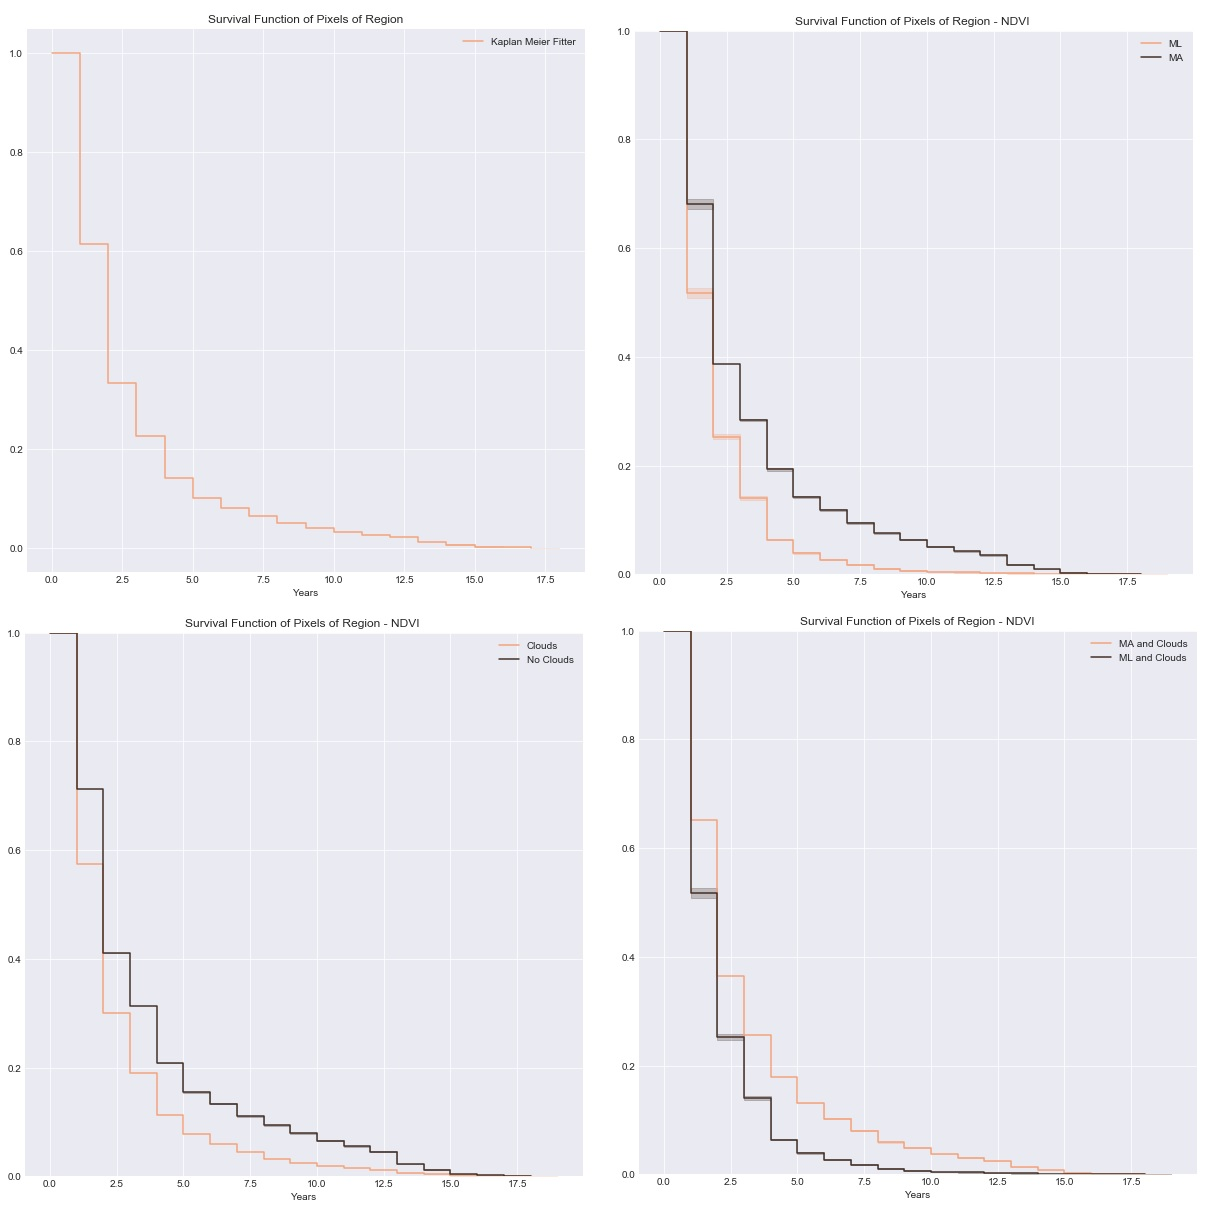
\includegraphics[width=1\textwidth]{KM_NDVI_complete.jpg}
\caption{Kaplan Meier Fitter for NDVI values in Region (LM+MA)}
\label{fig:km-total}
\end{figure}

\begin{table}[H]
\footnotesize
\caption{Kaplan Meier Estimation}
\begin{tabularx}{\linewidth}{l XXXXXX}
\hline
\hline
Time	&	Numbers at risk	&	Number of events	&	Survival 	&	Standard Errors  & lower 95\% CI & upper 95\% CI \\
\hline
Region  &&&&&& \\	
2001	&	512017	&	197454	&	0.61436	&	6.80E-04	&	0.61303	&	0.6157	\\
2005	&	71707	&	263281	&	0.10016	&	4.20E-04	&	0.09934	&	0.10098	\\
2011	&	20594	&	34998	&	0.0318	&	2.45E-04	&	0.03133	&	0.03229	\\
2015	&	3189	&	15180	&	0.00216	&	6.48E-05	&	0.00203	&	0.00229	\\
\hline
Region MA &&&&&& \\												\\
2001	&	302075	&	96251	&	0.68137	&	0.000848	&	0.6797	&	0.683	\\
2005	&	58271	&	162794	&	0.14245	&	0.000636	&	0.1412	&	0.1437	\\
2011	&	19179	&	27662	&	0.05087	&	0.0004	&	0.0501	&	0.0517	\\
2015	&	2946	&	14404	&	0.00319	&	0.000103	&	0.003	&	0.0034	\\
\hline
Region LM &&&&&& \\												\\
2001	&	209942	&	101203	&	0.517948	&	1.09E-03	&	0.515815	&	0.52009	\\
2005	&	13436	&	100487	&	0.039306	&	4.24E-04	&	0.038484	&	0.040146	\\
2011	&	1415	&	7336	&	0.004363	&	1.44E-04	&	0.00409	&	0.004654\\
2015	&	243	&	776	&	0.000667	&	5.63E-05	&	0.000565	&	0.000787\\
\hline
\hline
\end{tabularx}%
\label{tab:KM_estimate}%
\end{table}%

%MA
For the Cerrado Maranhão (MA), the Kaplan Meier fitter shows that from the 315,904 pixels, in 2001, between 64\% to 68\% of pixels had a chance of survival considering both vegetation indices. For 2010, the chance of survival decreased to the range of 3\% to 5\%. At the end of the studied period, the chance of survival for pixels within Cerrado Maranhão was around 0.3\% (see upper left graph from Figure \ref{fig:km-evi} and Figure \ref{fig:km-ndvi}, and Table \ref{tab:KM_estimate}). The median time of survival for the model was two years. This means that the half life of the sample pixels was around two years (the 50th percentile).

%MA + clouds 

Sub-setting the survival curves by the presence of Clouds, it's possible to identify that pixels with no clouds in the studied period had a higher rate of survival comparing to pixels with clouds. At the end of 2001, the rate of survival for pixels with no clouds was about 66.6\% to 71.2\% for both indices. In 2005, the rate lowered to around 15\% and, in 2015, the chance of survival of the forests was approximately 0.4\%. Looking to the survival curve of pixels covered by clouds, the chance of forest survival at 2001 was around 61\% to 65\%, then decreased to 11\% and 13\% in 2005. The rate of survival for forests in 2015 was around 0.2\% for both vegetation indices (see upper right graph from Figure \ref{fig:km-evi} and Figure \ref{fig:km-ndvi} ). The median time of survival for the survival curves stratified by clouds did not change from the original set. 


%Log Rank test on MA clouds

It was conducted a Log Rank test \citep{Peto_1972} to check whether these two sub samples were originated from the same distribution and the differences from these curves were resulted from other characteristics than the presence of clouds. The results showed that, in fact, these sub samples come from different distributions which allows to say that the differences are significant. Since the majority of the pixels are deforested within two years, it is also applied the generalized Wilcoxon test, which can be also referred to Log Rank Weighted test, because it gives more weight to early deforestation than later deforestation, while Log Rank test gives equal weight to all deforestation process \citep{lee_wang_2003}. The results reinforce that two survival curves are different from each other.

%ML + %ML + clouds
The Legal Maranhão (LM) experienced a similar pattern in which the median time of survival of the pixels was two years. From the 213,776 pixels analysed, approximately 51\% of the total had a chance of survival in 2001. This rate drops to about 4\% in 2005 and, ten years later, to 0.06\%. It appears from the survival curve that the rate of survival was lower for the Legal Maranhão (LM). Stratifying by clouds, the survival curves show that pixels without the presence of clouds had a higher rater of survival for both indices (see lower right graph from Figure \ref{fig:km-evi} and Figure \ref{fig:km-ndvi}). The rate of survival for pixels with no clouds was about 58.8\% to 59.2\% in 2001. Then, the rate dropped to around 2.5\% in 2010 and no rate for survived pixels in 2015. The chance of survival for pixels covered by clouds was around 51\% in 2001 for both indices, almost 10\% lower when comparing with not clouded pixels. In 2010, the rate of survival was less than 0.5\% and, in 2015, was equivalent to 0.065\%. 

%Log Rank test on ML clouds
It was performed the Log Rank test \citep{Peto_1972} to check whether the two sub samples were originated from the same distribution and the differences from these survival curves were due to other characteristics than the presence of clouds. The test result showed that the two sub samples are from different distributions. It was also applied the generalized Wilcoxon test \citep{lee_wang_2003} which rejected the null hypothesis that the two series came from the same distribution origin. 

\begin{figure}[H]
  \centering
  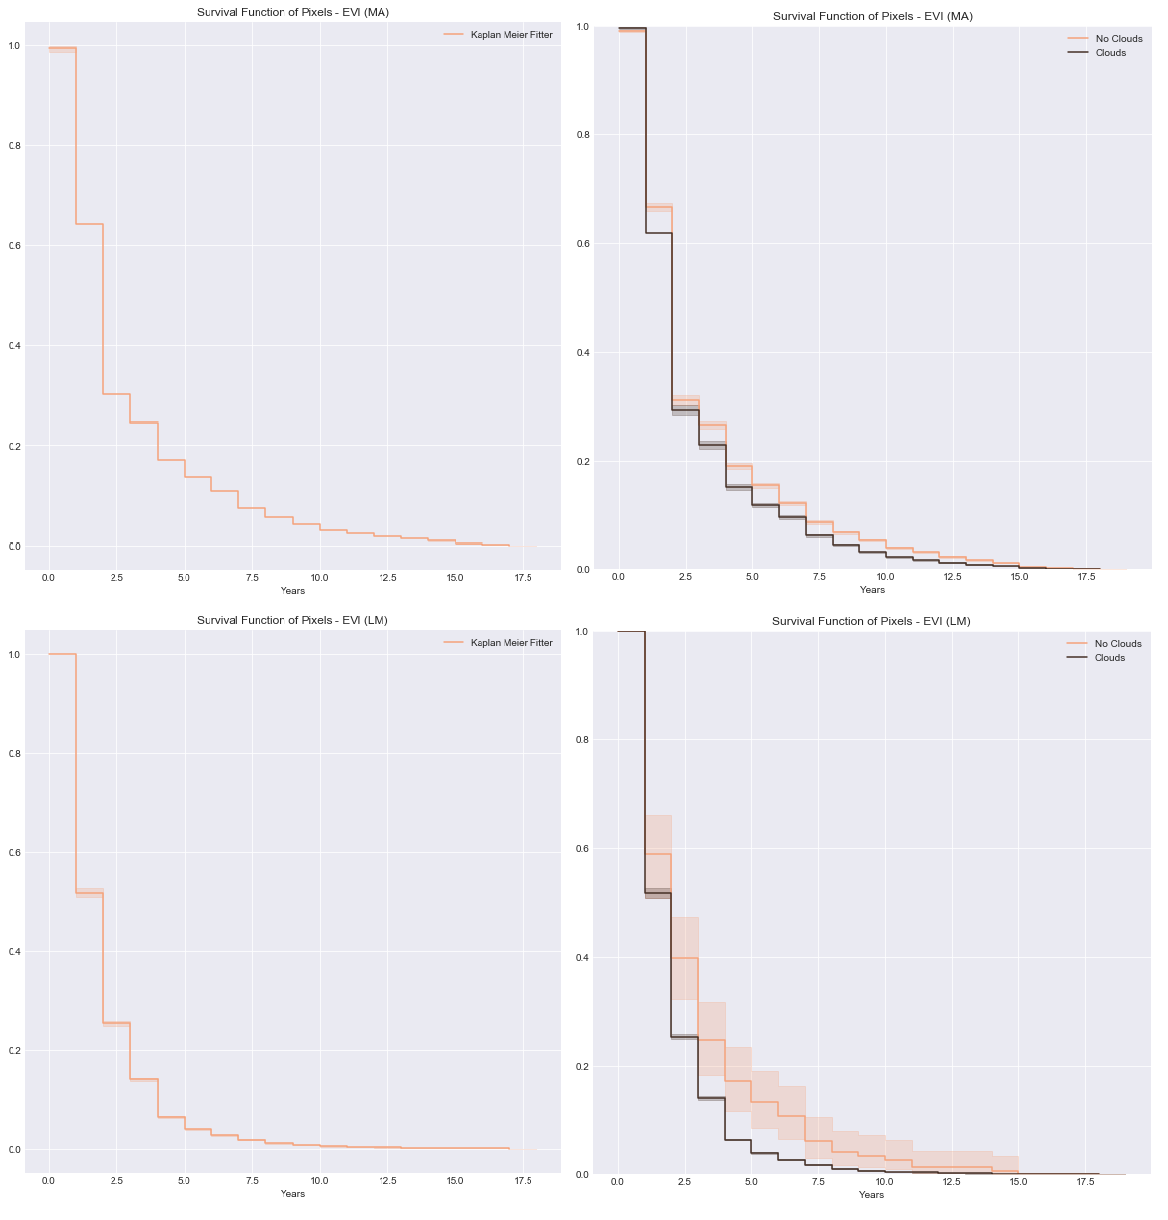
\includegraphics[width=1\textwidth]{KM_EVI.png}
\caption{Kaplan Meier Fitter for EVI values in LM and MA region}
\label{fig:km-evi}
\end{figure}

\begin{figure}[H]
  \centering
  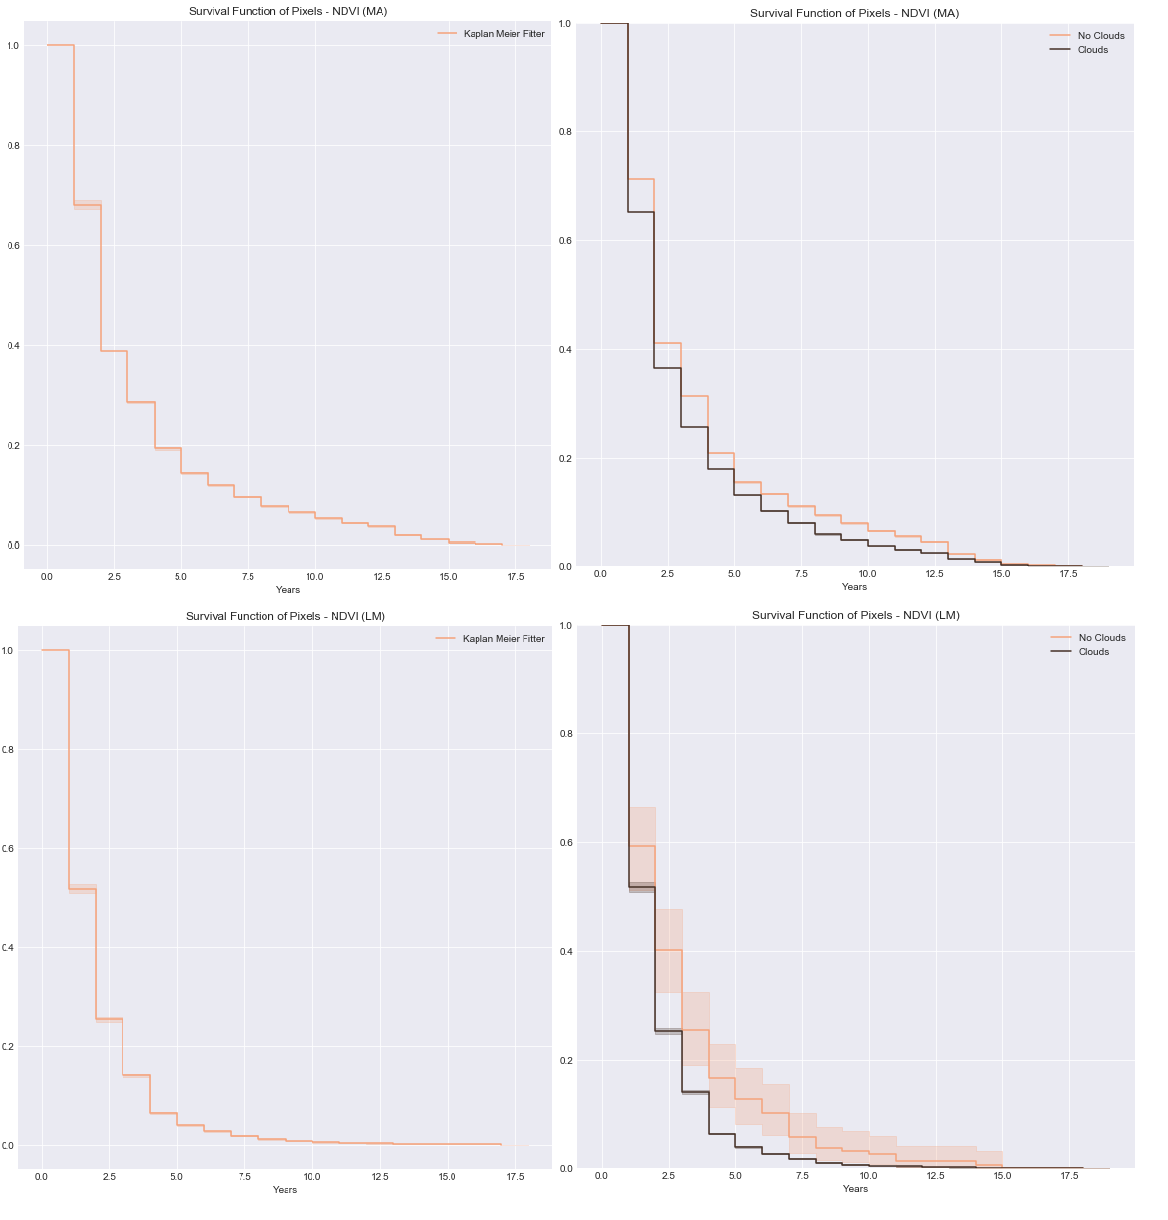
\includegraphics[width=1\textwidth]{KM_NDVI.png}
\caption{Kaplan Meier Fitter for NDVI values in LM and MA region}
\label{fig:km-ndvi}
\end{figure}


\subsection{Semi parametric Analysis} \label{resultssection2}

%MA + ML
Studying forest loss and, in consequence, deforestation reveals that many factors potentially affect the process. In this sense, we expand the analysis to include risk factors and covariates to evaluate the effect of these variables on forest survival (see \ref{eq:6}). 

Starting the analysis looking to the whole Region, the preferred model was the NDVI model considering the concordance index (0.755) and k-fold model validation (0.03). This approach allowed to interact cloud cover and region, in principle, our interest variable. Table \ref{tab:CPH_NDVI_MA_ML} evidences the regression coefficients, their standard errors, the z values, and relative hazards or relative risks, such as Clouds, Protected Areas, Mining, Elevation, Markets, Municipalities centre, Rivers and Roads. Latitude and longitude are controls to the model along with grouped year periods. From the results, elevation has no effect on relative hazard. The presence of clouds increases hazard by 1.5\%. Distancing from protected areas and paved roads decrease hazard by 4.7\% and 23.8\%, respectively. On the other hand, distancing from markets and municipalities centre increase hazard by 6.5\% and 19.1\%. Clouds are not significant, however the fact the pixel is in the Legal Maranhão side increases hazard by 29.4\%. 
%MA + ML Diagnostics

For this model, we check the proportional hazard assumption with plots of each estimated regression coefficient as a function of time through the smoothed scaled Schoenfeld residuals. The results showed that each risk factor curve presents a flat format suggesting that the proportional hazard assumption holds. To access the goodness of fit of this model, we plotted the graph of deviance residuals against the survival time. The results showed that the residuals were distributed about zero showing a good fit of the model. 

\begin{table}[H]
\footnotesize
\caption{Cox Proportional Hazard Model - Region}
\begin{tabularx}{\linewidth}{X YYYYY}
\hline
\hline
Variables	&	Regression Coefficient	&	Relative Hazards	&	Standard Errors	&	z score & Pr (>|z|) \\
\hline
Clouds	&	0.015	&	1.015	&	0.004	&	3.634	&	3E-04	***	\\	
Pas	&	-0.049	&	0.953	&	0.010	&	-4.912	&	9E-07	***	\\	
Mining	&	0.340	&	1.405	&	0.022	&	15.633	&	<	2E-16	***	\\
Elevation	&	0.001	&	1.001	&	0.003	&	0.173	&	0.86		\\	
Markets	&	0.063	&	1.065	&	0.010	&	5.998	&	2E-09	***	\\	
Municipalities	&	0.175	&	1.191	&	0.026	&	6.842	&	8E-12	***	\\	
Rivers	&	0.252	&	1.286	&	0.114	&	2.199	&	0.03	*	\\	
Roads	&	-0.271	&	0.762	&	0.043	&	-6.250	&	4E-10	***	\\	
Lat	&	-0.074	&	0.929	&	0.004	&	-19.147	&	<	2E-16	***	\\
Lon	&	0.254	&	1.290	&	0.013	&	19.407	&	<	2E-16	***	\\
Region	&	0.258	&	1.294	&	0.080	&	3.220	&	1E-03	**	\\	
Cloud*Region	&	0.089	&	1.093	&	0.080	&	1.107	&	0.27 \\	
\hline
\hline
\multicolumn{6}{l}{Signs stand for '***' 0.001 '**' 0.01 '*' 0.05 '.' 0.1 and denote hazard ratios that are significantly}\\
\multicolumn{6}{l}{ different from 1 at 99\%, 95\% and 90\% confidence levels. The model contains controls for grouped year}\\
\multicolumn{6}{l}{periods. PAs stand for Protected Areas (Indigenous Lands and Conservational Units).}\\
\end{tabularx}%
\label{tab:CPH_NDVI_MA_ML}%
\end{table}%


%MA and %MA Diagnostics

Sub-setting the sample to analyse the Cerrado Maranhão (MA), the NDVI model was preferred in many settings when accounting for concordance index (0.767) and k-fold model validation (0.30) (see Table \ref{kfold}. Table \ref{tab:CPH_NDVI_MA} shows the results of the specified model. Pixels covered by clouds decreases the risk of the pixel being deforested by 2\% compared to those pixels not covered by clouds. Pixels far from rivers increase relative hazard by 55\%. Distancing one unit from protected areas, the risk of deforestation increases by 4\%, the same occurs with mines with a increase of 32\% in the relative hazard. Distancing one unit from markets and municipalities increase hazard by 6\% and 8\%. However, distancing one unit from roads decreases the relative risk of the pixels been deforested in that area by 48\%. The diagnostics of the model corroborates to the assumption of proportional hazard during the studied period and the deviance residuals exhibit a good fit. 

\begin{table}[H]
\footnotesize
\caption{Cox Proportional Hazard Model - Cerrado Maranhão (MA)}
\begin{tabularx}{\linewidth}{X YYYYY}
\hline
\hline
Variables	&	Regression Coefficient	&	Relative Hazards	&	Standard Errors	&	z score & Pr (>|z|) \\
\hline
Clouds	&	-0.015	&	0.98	&	0.004	&	-3.65	&	3E-04	***	\\	
PAs	&	0.036	&	1.04	&	0.017	&	2.05	&	0.041	*	\\	
Mining	&	0.275	&	1.32	&	0.028	&	10.00	&	<	2E-16	***	\\
Elevation	&	0.020	&	1.02	&	0.005	&	4.18	&	3E-05	***	\\	
Markets	&	0.061	&	1.06	&	0.017	&	3.48	&	0.001	***	\\	
Municipalities	&	0.077	&	1.08	&	0.033	&	2.34	&	0.019	*	\\	
Rivers	&	0.436	&	1.55	&	0.150	&	2.90	&	0.004	**	\\	
Roads	&	-0.660	&	0.52	&	0.052	&	-12.61	&	<	2E-16	***	\\
Lat	&	-0.149	&	0.86	&	0.007	&	-21.59	&	<	2E-16	***	\\
Lon	&	0.258	&	1.29	&	0.017	&	15.21	&	<	2E-16	***	\\
\hline
\hline
\multicolumn{6}{l}{Signs stand for '***' 0.001 '**' 0.01 '*' 0.05 '.' 0.1 and denote hazard ratios that are significantly }\\
\multicolumn{6}{l}{different from 1 at 99\%, 95\% and 90\% confidence levels. The model contains controls for grouped year}\\
\multicolumn{6}{l}{periods. PAs stand for Protected Areas. Indigenous Lands and Conservational Units.}\\
\end{tabularx}%
\label{tab:CPH_NDVI_MA}%
\end{table}%


%Teve que stratificar a analise para 3 cortes no tempo de 2000 a 2002, 2002 a 2005, 2005 a 2016. teve que fazer isso pq o teste PH assumiu que os fatores de riscos!!!

%ML and %ML Diagnostics
Following the same selection procedure adopted to the previous model, the two vegetation indices models for Legal Maranhão (LM) the NDVI model presented was favoured considering the c-index and the k-fold validation. Table \ref{tab:CPH_NDVI_ML} shows the results of the proportional hazard model for the Maranhão region under environmental policy (LM). Clouds are not significant in this model and elevation has a constant effect on the relative hazard. Distancing one unit from protected areas, the risk of deforestation increases by almost 9\%. However, distancing from river basins decreases hazard by approximately 34\%. Distancing from roads in the policy area increases hazard by 25\%. The Legal Maranhão (LM) deviance residuals showed that the model presents a good fit with no pattern detected. The scaled Schoenfeld residuals also show a flat curve for all the risk factor variables. These results hold the assumption of the proportional hazard model.

\begin{table}[H]
\footnotesize
\caption{Cox Proportional Hazard Model - Legal Maranhão (LM)}
\begin{tabularx}{\linewidth}{X YYYYY}
\hline
\hline
Variables	&	Regression Coefficient	&	Relative Hazards	&	Standard Errors	&	z score & Pr (>|z|) \\
\hline
Clouds	&	0.108	&	1.113	&	0.080	&	1.344	&	0.179			\\
PAs	&	0.081	&	1.084	&	0.016	&	5.137	&	3E-07	***		\\
Mining	&	-0.019	&	0.981	&	0.049	&	-0.387	&	0.699			\\
Elevation	&	-0.011	&	0.989	&	0.004	&	-2.498	&	0.012	*		\\
Markets	&	-0.023	&	0.977	&	0.015	&	-1.588	&	0.112			\\
Municipalities	&	-0.070	&	0.932	&	0.045	&	-1.562	&	0.118			\\
Rivers	&	-0.413	&	0.662	&	0.179	&	-2.307	&	0.021	*		\\
Roads	&	0.224	&	1.251	&	0.085	&	2.645	&	0.008	**		\\
Lat	&	-0.046	&	0.955	&	0.006	&	-8.218	&	2E-16	***		\\
Lon	&	0.282	&	1.325	&	0.025	&	11.396	&	<	2E-16	***	\\
\hline
\hline
\multicolumn{6}{l}{Signs stand for '***' 0.001 '**' 0.01 '*' 0.05 '.' 0.1 and denote hazard ratios that are significantly }\\
\multicolumn{6}{l}{different from 1 at 99\%, 95\% and 90\% confidence levels. The model contains controls for grouped year}\\
\multicolumn{6}{l}{periods. PAs stand for Protected Areas. Indigenous Lands and Conservational Units.}\\
\end{tabularx}%
\label{tab:CPH_NDVI_ML}%
\end{table}%

%\subsubsection{Extended Cox Proportional Hazard Model}

%CoxPH Time Dependent MA + ML
Until this moment, the proportional hazards models are assumed to have risk factors independent of time. However, in practice, deforestation is a process that might have spatially time dependent factors. In this sense, we extend the Cox proportional Hazard model for the Region and sampled areas. 

To incorporate the spatially and temporal dependence, we include the ratio of neighbouring forested pixels for each pixel in four different periods (2001, 2006, 2011, 2016). We also include average values of rainfall and temperature distributed within the specified years and interact them with policy region of Legal Maranhão. Table \ref{tab:CPH_NDVI_MA_ML_time} shows the results from this setting. Clouds increase the chance of deforestation by 1.8\%. Distancing one unit from protected areas decreases hazard by 4.4\%. Distancing one unit from mines, increase hazard by 20\% and elevated areas increased hazard by 3.5\%. Distancing from roads decrease hazard by almost 18\%. Clouded pixels in the Legal Maranhão region does not have an effect on hazard. Observing the time dependent variables, having neighbouring pixels with forest increase the risk of being cleared by 31\%. Increasing rainfall and temperature in the whole region decreases hazard by 0.1\%. Finally, rainfall and temperature in the Legal Maranhão side has a different outcome for rainfall. High levels of precipitation increases hazard by 0.1\% and increasing temperature decreases hazard by 1.4\%. 

\begin{table}[H]
\footnotesize
\caption{Cox Proportional Hazard Model Time Dependent - Region}
\begin{tabularx}{\linewidth}{X YYYYY}
\hline
\hline
Variables	&	Regression Coefficient	&	Relative Hazards	&	Standard Errors	&	z score & Pr (>|z|) \\
\hline
Clouds	&	0.018	&	1.018	&	0.01	&	3.20	&	0.001	**	\\	
Pas	&	-0.045	&	0.956	&	0.01	&	-3.07	&	0.002	**	\\	
Mining	&	0.187	&	1.205	&	0.03	&	6.40	&	2E-10	***	\\	
Elevation	&	0.034	&	1.035	&	0.00	&	8.42	&	<	2E-16	***	\\
Markets	&	0.024	&	1.025	&	0.02	&	1.56	&	0.118		\\	
Municipalities	&	-0.057	&	0.945	&	0.03	&	-1.66	&	0.097	.	\\	
Rivers &	-0.452 &	0.637 &	0.155 &	-2.915 &	0.003	** \\
Roads	&	-0.197	&	0.821	&	0.06	&	-3.36	&	0.001	***	\\	
Lat	&	0.000	&	1.000	&	0.01	&	-0.06	&	0.952		\\	
Lon	&	-0.034	&	0.966	&	0.02	&	-2.05	&	0.041	*	\\	
Region	&	0.293	&	1.341	&	0.10	&	3.06	&	0.002	**	\\	
Cloud*Region	&	0.018	&	1.018	&	0.01	&	1.52	&	0.130		\\	
Neighbours	&	0.274	&	1.315	&	0.03	&	10.44	&	<	2E-16	***	\\
Rainfall	&	-0.001	&	0.999	&	0.00	&	-6.47	&	1E-10	***	\\	
Rainfall*Region	&	0.001	&	1.001	&	0.00	&	6.61	&	4E-11	***	\\	
Temperature	&	-0.006	&	0.994	&	0.00	&	-2.28	&	2E-02	*	\\	
Temperature*Region	&	-0.014	&	0.986	&	0.00	&	-5.36	&	8E-08	***	\\	
\hline
\hline
\multicolumn{6}{l}{Signs stand for '***' 0.001 '**' 0.01 '*' 0.05 '.' 0.1 and denote hazard ratios that are significantly }\\
\multicolumn{6}{l}{different from 1 at 99\%, 95\% and 90\% confidence levels. The model contains controls for grouped and }\\
\multicolumn{6}{l}{time-dependent year periods. PAs stand for Protected Areas. Indigenous Lands and Conservational Units.}\\
\end{tabularx}%
\label{tab:CPH_NDVI_MA_ML_time}%
\end{table}%


%CoxPH Time Dependent MA 
We applied the same procedure to both areas apart. Cerrado Maranhão (MA) results are presented in Table \ref{tab:CPH_NDVI_MA_time} and Legal Maranhão (LM) results are shown in Table \ref{tab:CPH_NDVI_ML_time}. The results from the area not monitored shows that the presence of Clouds has no effect on the relative hazard. Forested pixels distant from protected areas decreases the risk of being deforested by 18\%. Distancing from roads and rivers also decreases hazard by 23\% and 33\%. Looking to the time dependent controls, we can see that forested pixels surrounded by forest increase 2 time the relative hazard. Rainfall decreases the risk of the pixel being deforested by 0.1\% and high temperature increases the chance of deforestation by 6.3\%. 

\begin{table}[H]
\footnotesize
\caption{Cox Proportional Hazard Model Time Dependent - Cerrado Maranhão (MA)}
\begin{tabularx}{\linewidth}{X YYYYY}
\hline
\hline
Variables	&	Regression Coefficient	&	Relative Hazards	&	Standard Errors	&	z score & Pr (>|z|) \\
\hline
Clouds	&	0.003	&	1.003	&	0.006	&	0.534	&	0.593		\\	
PAs	&	-0.207	&	0.814	&	0.024	&	-8.446	&	<	2E-16	***	\\
Mining	&	0.055	&	1.057	&	0.041	&	1.352	&	0.176	\\		
Elevation	&	0.066	&	1.069	&	0.006	&	10.581	&	<	2E-16	***	\\
Markets	&	0.177	&	1.193	&	0.026	&	6.881	&	6E-12	***	\\	
Municipalities	&	-0.243	&	0.784	&	0.045	&	-5.373	&	8E-08	***	\\	
Rivers	&	-0.455	&	0.635	&	0.204	&	-2.232	&	0.026	*	\\	
Roads	&	-0.269	&	0.764	&	0.072	&	-3.713	&	2E-04	***	\\	
Lat	&	-0.282	&	0.755	&	0.011	&	-24.792	&	<	2E-16	***	\\
Lon	&	0.155	&	1.167	&	0.025	&	6.180	&	6E-10	***	\\	
Neighbours	&	0.742	&	2.099	&	0.040	&	18.379	&	<	2E-16	***	\\
Rainfall	&	-0.009	&	0.991	&	0.000	&	-26.481	&	<	2E-16	***	\\
Temperature	&	0.062	&	1.063	&	0.003	&	19.476	&	<	2E-16	***	\\
\hline
\hline
\multicolumn{6}{l}{Signs stand for '***' 0.001 '**' 0.01 '*' 0.05 '.' 0.1 and denote hazard ratios that are significantly }\\
\multicolumn{6}{l}{different from 1 at 99\%, 95\% and 90\% confidence levels. The model contains controls for grouped and}\\
\multicolumn{6}{l}{time-dependent year periods. PAs stand for Protected Areas. Indigenous Lands and Conservational Units.}\\
\end{tabularx}%
\label{tab:CPH_NDVI_MA_time}%
\end{table}%

%CoxPH Time Dependent ML
In the surveilled area, Table \ref{tab:CPH_NDVI_ML_time} indicates that the pattern differs from the previous result. The presence of clouds increase the risk of a pixel being deforested by 3\%. Distancing one unit from markets and mining projects increases hazard by 9.7\% and 1.6\%, accordingly Being located to neighbouring forested pixels increases hazard by 33\% and the increasing level of temperature decreases the relative risk of a pixel being deforested by 2.1\%.

\begin{table}[H]
\footnotesize
\caption{Cox Proportional Hazard Model Time Dependent - Legal Maranhão (LM)}
\begin{tabularx}{\linewidth}{X YYYYY}
\hline
\hline
Variables	&	Regression Coefficient	&	Relative Hazards	&	Standard Errors	&	z score & Pr (>|z|) \\
\hline
Clouds	&	0.030	&	1.030	&	0.011	&	2.592	&	0.010	**		\\
Pas	&	-0.060	&	0.941	&	0.020	&	-3.055	&	0.002	**		\\
Mining	&	0.175	&	1.191	&	0.050	&	3.518	&	4E-04	***		\\
Elevation	&	0.016	&	1.016	&	0.006	&	2.724	&	0.006	**		\\
Markets	&	0.093	&	1.097	&	0.021	&	4.497	&	7E-06	***		\\
Municipalities	&	-0.102	&	0.903	&	0.054	&	-1.901	&	0.057	.		\\
Rivers	&	-0.090	&	0.914	&	0.241	&	-0.374	&	0.708			\\
Roads	&	0.026	&	1.026	&	0.103	&	0.252	&	0.801			\\
Lat	&	0.034	&	1.034	&	0.008	&	4.149	&	3E-05	***		\\
Lon	&	-0.145	&	0.865	&	0.027	&	-5.338	&	9E-08	***		\\
Neighbours	&	0.289	&	1.335	&	0.034	&	8.37	&	<	2E-16	***	\\
Rainfall	&	0.000	&	1.000	&	0.000	&	1.075	&	0.283			\\
Temperature	&	-0.021	&	0.979	&	0.001	&	-20.965	&	<	2E-16	***	\\
\hline
\hline
\multicolumn{6}{l}{Signs stand for '***' 0.001 '**' 0.01 '*' 0.05 '.' 0.1 and denote hazard ratios that are significantly }\\
\multicolumn{6}{l}{different from 1 at 99\%, 95\% and 90\% confidence levels. The model contains controls for grouped and}\\
\multicolumn{6}{l}{time-dependent year periods. PAs stand for Protected Areas. Indigenous Lands and Conservational Units.}\\
\end{tabularx}%
\label{tab:CPH_NDVI_ML_time}%
\end{table}%

\subsection{Different areas different results? Robustness Checks} \label{resultssection2.1}

\subsubsection{Buffer Zone}
We decide to deepen our analysis by expanding the area to immediately outside the studied region. We constructed a buffer of 0.2 decimal degrees which corresponds to our average maximum reach of our risk factors in the Region. We exclude the area previously analysed to check if the results are consistently different from our findings. We believe that the uniqueness of our findings comes from the fact that the two areas (MA and LM) are similar in all aspects except from the implementation of the environmental policy. 

We first approach with the non parametric analysis. The Kaplan Meier fitter shows that the chance of survival of the forests through the analysis of pixels was higher in the Legal Maranhão (LM) than in Cerrado Maranhão (MA) (upper right from Graph \ref{fig:km-total-buffer}). From the 91,346 pixels observations, the rate of survival for the pixels in the buffer region was about 55\% in 2001 and, in 2005, the rate of survival decreased to approximately 8\%. In 2015, the rate was equivalent to 0.25\%. The Log Rank test and Weighted Log Rank test confirms that the stratified sample differs in terms of distribution. Dividing the sample by region, it's possible to identify that pixels within Legal Maranhão buffer (LM) had a higher rate of survival comparing to pixels within Cerrado Maranhão buffer (MA). This result differs from our findings for the Region. The presence of clouds in this subset still shows that the chance of survival was higher in the Legal Maranhão (LM) side, see lower right in Graph \ref{fig:km-total-buffer}. 

\begin{figure}[H]
  \centering
  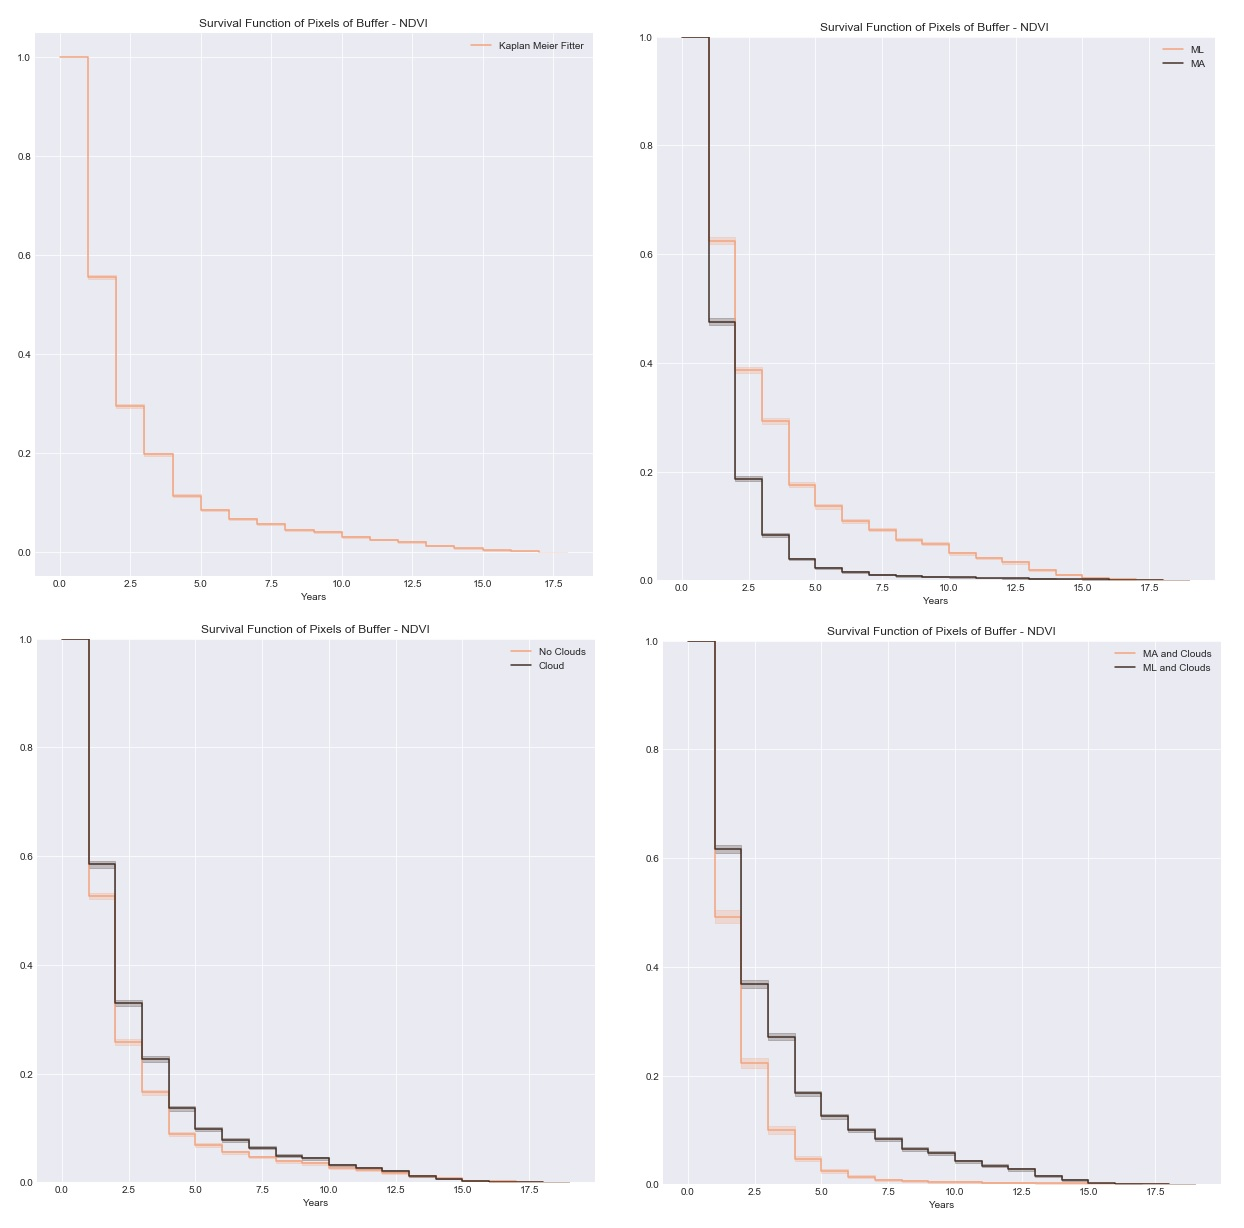
\includegraphics[width=1\textwidth]{KM_NDVI_buffer_total.jpg}
\caption{Kaplan Meier Fitter for NDVI values in Buffer Zone}
\label{fig:km-total-buffer}
\end{figure}


Table \ref{tab:CPH_NDVI_buffer} presents the results for the semiparametric model and Table \ref{tab:CPH_NDVI_buffer_time} shows the time dependent version of the specified model. Within the buffer zone, the presence of clouds has a negative impact on the risk of a pixel being deforested, the hazard decreases by 3\%. Distancing from protected areas increases hazard by 35\% and distancing from markets, municipalities centre and rivers decreases hazard by 18\%, 19\% and 61\%. The fact that the pixel is located in the buffer zone within the Legal Maranhão decreases the relative risk of clear cutting by 33\%. However, the presence of clouds in this same area increases hazard in 6\% comparing to pixels outside the limits. As with the sample area, we extend the model to account for changes in time. After controlling for spatial and temporal aspects, the results indicate that the presence of clouds conditioning on the surveilled area has no effect on the relative hazard. Region is still negative and significant. The relative hazard decreases in almost 99\% for pixels in the Legal Maranhão (LM). For the same area, increasing temperature and rainfall increases hazard by 0.2\% and 7\%, respectively.

%Falar do teste cohens
The results seem to differ from the original area (Figure \ref{fig:delimitacao}) and to endorse our findings we conduct a effect size measure for the two areas: the region and the buffer zone. Based on \citet{COHEN1977} we take differences of means expressed in terms of the pooled within regions standard deviation. Unlike significance tests, this index is independent of sample size. The pooled standard deviation is the square root of the average of the squared standard deviation of the two areas. According to \citet{COHEN1977}, if the two standard deviations are similar the root mean square will not differ much from the simple average of the two variances. In our setting, the Cohen Index is interpreted in terms of of the average percentile standing of the Region relative to the buffer zone. An index of 0.0 indicates that the mean of the Region is at the 50th percentile of the buffer zone, i.e the dissimilarities for the two areas are zero. In our results, the Cohen index presented a value of 0.59 which configures that the Region is at the 69th percentile of the buffer zone and thus these areas present substantial dissimilarities. We reject the null hypothesis that there is no difference between these groups. Effect sizes can also be interpreted in terms of the percent of distinction of one region score to another. A Cohen index of 0 indicates that the distribution of scores for one region overlaps completely with the distribution of scores of another region, there is 0\% of distinction. In our case, the index of 0.59 indicates a distinction of 33\% in the two distributions \citep{COHEN1977}.

\begin{table}[H]
\footnotesize
\caption{Cox Proportional Hazard Model - Buffer Zone}
\begin{tabularx}{\linewidth}{X YYYYY}
\hline
\hline
Variables	&	Regression Coefficient	&	Relative Hazards	&	Standard Errors	&	z score & Pr (>|z|) \\
\hline
Clouds	&	-0.036	&	0.965	&	0.016	&	-2.183	&	0.029	*		\\
PAs	&	0.297	&	1.350	&	0.024	&	12.189	&	<	0.000	***	\\
Mining	&	-0.314	&	0.730	&	0.045	&	-7.021	&	0.000	***		\\
Elevation	&	0.000	&	1.000	&	0	&	-3.610	&	0.000	***		\\
Markets	&	-0.202	&	0.817	&	0.024	&	-8.358	&	<	0.000	***	\\
Municipalities	&	-0.207	&	0.813	&	0.077	&	-2.697	&	0.007	**		\\
Rivers	&	-0.934	&	0.393	&	0.322	&	-2.899	&	0.004	**		\\
Roads	&	-0.113	&	0.893	&	0.142	&	-0.793	&	0.428			\\
Lat	&	-0.122	&	0.885	&	0.047	&	-2.593	&	0.010	**		\\
Lon	&	0.094	&	1.100	&	0.008	&	11.562	&	<	0.000	***	\\
Region	&	-0.407	&	0.666	&	0.033	&	-12.212	&	<	0.000	***	\\
Clouds*Region	&	0.058	&	1.060	&	0.021	&	2.726	&	0.006	**		\\
\hline
\hline
\multicolumn{6}{l}{Signs stand for '***' 0.001 '**' 0.01 '*' 0.05 '.' 0.1 and denote hazard ratios that are significantly}\\
\multicolumn{6}{l}{ different from 1 at 99\%, 95\% and 90\% confidence levels. The model contains controls for grouped year}\\
\multicolumn{6}{l}{periods. PAs stand for Protected Areas. Indigenous Lands and Conservational Units.}\\
\end{tabularx}%
\label{tab:CPH_NDVI_buffer}%
\end{table}%

\begin{table}[H]
\footnotesize
\caption{Cox Proportional Hazard Model Time Dependent - Buffer Zone}
\begin{tabularx}{\linewidth}{X YYYYY}
\hline
\hline
Variables	&	Regression Coefficient	&	Relative Hazards	&	Standard Errors	&	z score & Pr (>|z|) \\
\hline
Clouds	&	0.004	&	1.004	&	0.027	&	0.140	&	0.889			\\
PAs	&	0.146	&	1.157	&	0.039	&	3.698	&	2E-04	***		\\
Mining	&	0.141	&	1.152	&	0.067	&	2.112	&	0.035	*		\\
Elevation	&	0.000	&	1.000	&	0.000	&	-1.631	&	0.103			\\
Markets	&	-0.138	&	0.871	&	0.039	&	-3.518	&	4E-04	***		\\
Municipalities	&	-0.265	&	0.767	&	0.113	&	-2.343	&	0.019	*		\\
Rivers & -0.568	& 0.567 &	0.477 &	-1.191	& 0.234 \\
Roads	&	-0.174	&	0.841	&	0.207	&	-0.839	&	0.401			\\
Lat	&	0.072	&	1.074	&	0.042	&	1.703	&	0.089	.		\\
Lon	&	0.056	&	1.058	&	0.015	&	3.645	&	3E-04	***		\\
Region	&	-2.604	&	0.074	&	0.167	&	-15.627	&	<	2E-16	***	\\
Clouds*Region	&	-0.005	&	0.995	&	0.032	&	-0.167	&	0.867			\\
Neighbours	&	-0.041	&	0.960	&	0.031	&	-1.312	&	0.189			\\
Rainfall	&	-0.001	&	0.999	&	0.001	&	-1.422	&	0.155			\\
Rainfall*Region	&	0.002	&	1.000	&	0.001	&	3.150	&	0.002	**		\\
Temperature	&	0.003	&	1.003	&	0.003	&	0.896	&	0.370			\\
Temperature*Region	&	0.068	&	1.070	&	0.005	&	12.433	&	<	2E-16	***	\\
\hline
\hline
\multicolumn{6}{l}{Signs stand for '***' 0.001 '**' 0.01 '*' 0.05 '.' 0.1 and denote hazard ratios that are significantly }\\
\multicolumn{6}{l}{different from 1 at 99\%, 95\% and 90\% confidence levels. The model contains controls for grouped and }\\
\multicolumn{6}{l}{time-dependent year periods. PAs stand for Protected Areas. Indigenous Lands and Conservational Units.}\\
\end{tabularx}%
\label{tab:CPH_NDVI_buffer_time}%
\end{table}%


\subsubsection{Settlements} \label{resultssection3.1}

We have examined the Region (MA and LM), considering their spatial definition. To further investigate whether the environmental policy demonstrated to be effective under the presence of clouds we also look specifically to the survival time of forested pixels within settlements which are known to be allocated and supervised by Brazil’s Special Secretary of Agrarian Development, and there is virtually no law enforcement in these areas. Usually, the fines are sent to INCRA and not to the settler. Usually, the justice system claims that the agrarian agency does not commit an environmental crime because the agency leaves part of the forest of the whole settlement intact, but cannot oblige the granted slots to detain forest clearing. Under pressure by public opinion, INCRA established in 2012 the 'Green Settlement Program' to deal with the environmental debt of settlements. This policy, however, is still not implemented and there is no feasibility that could endorse the effectiveness of this policy \citet{PACHECO,PERES2}. Under these circumstances, and in an attempt to corroborate with the finding results, this study took from the observed region, settlements areas from both sides MA and ML (see figure \ref{fig:delimitacaosett} since they are not directly affected by any surveillance monitoring policy in order to check whether the time of survival of the pixels differed or was equal to the rest of the region.

\begin{figure}[H]
  \centering
  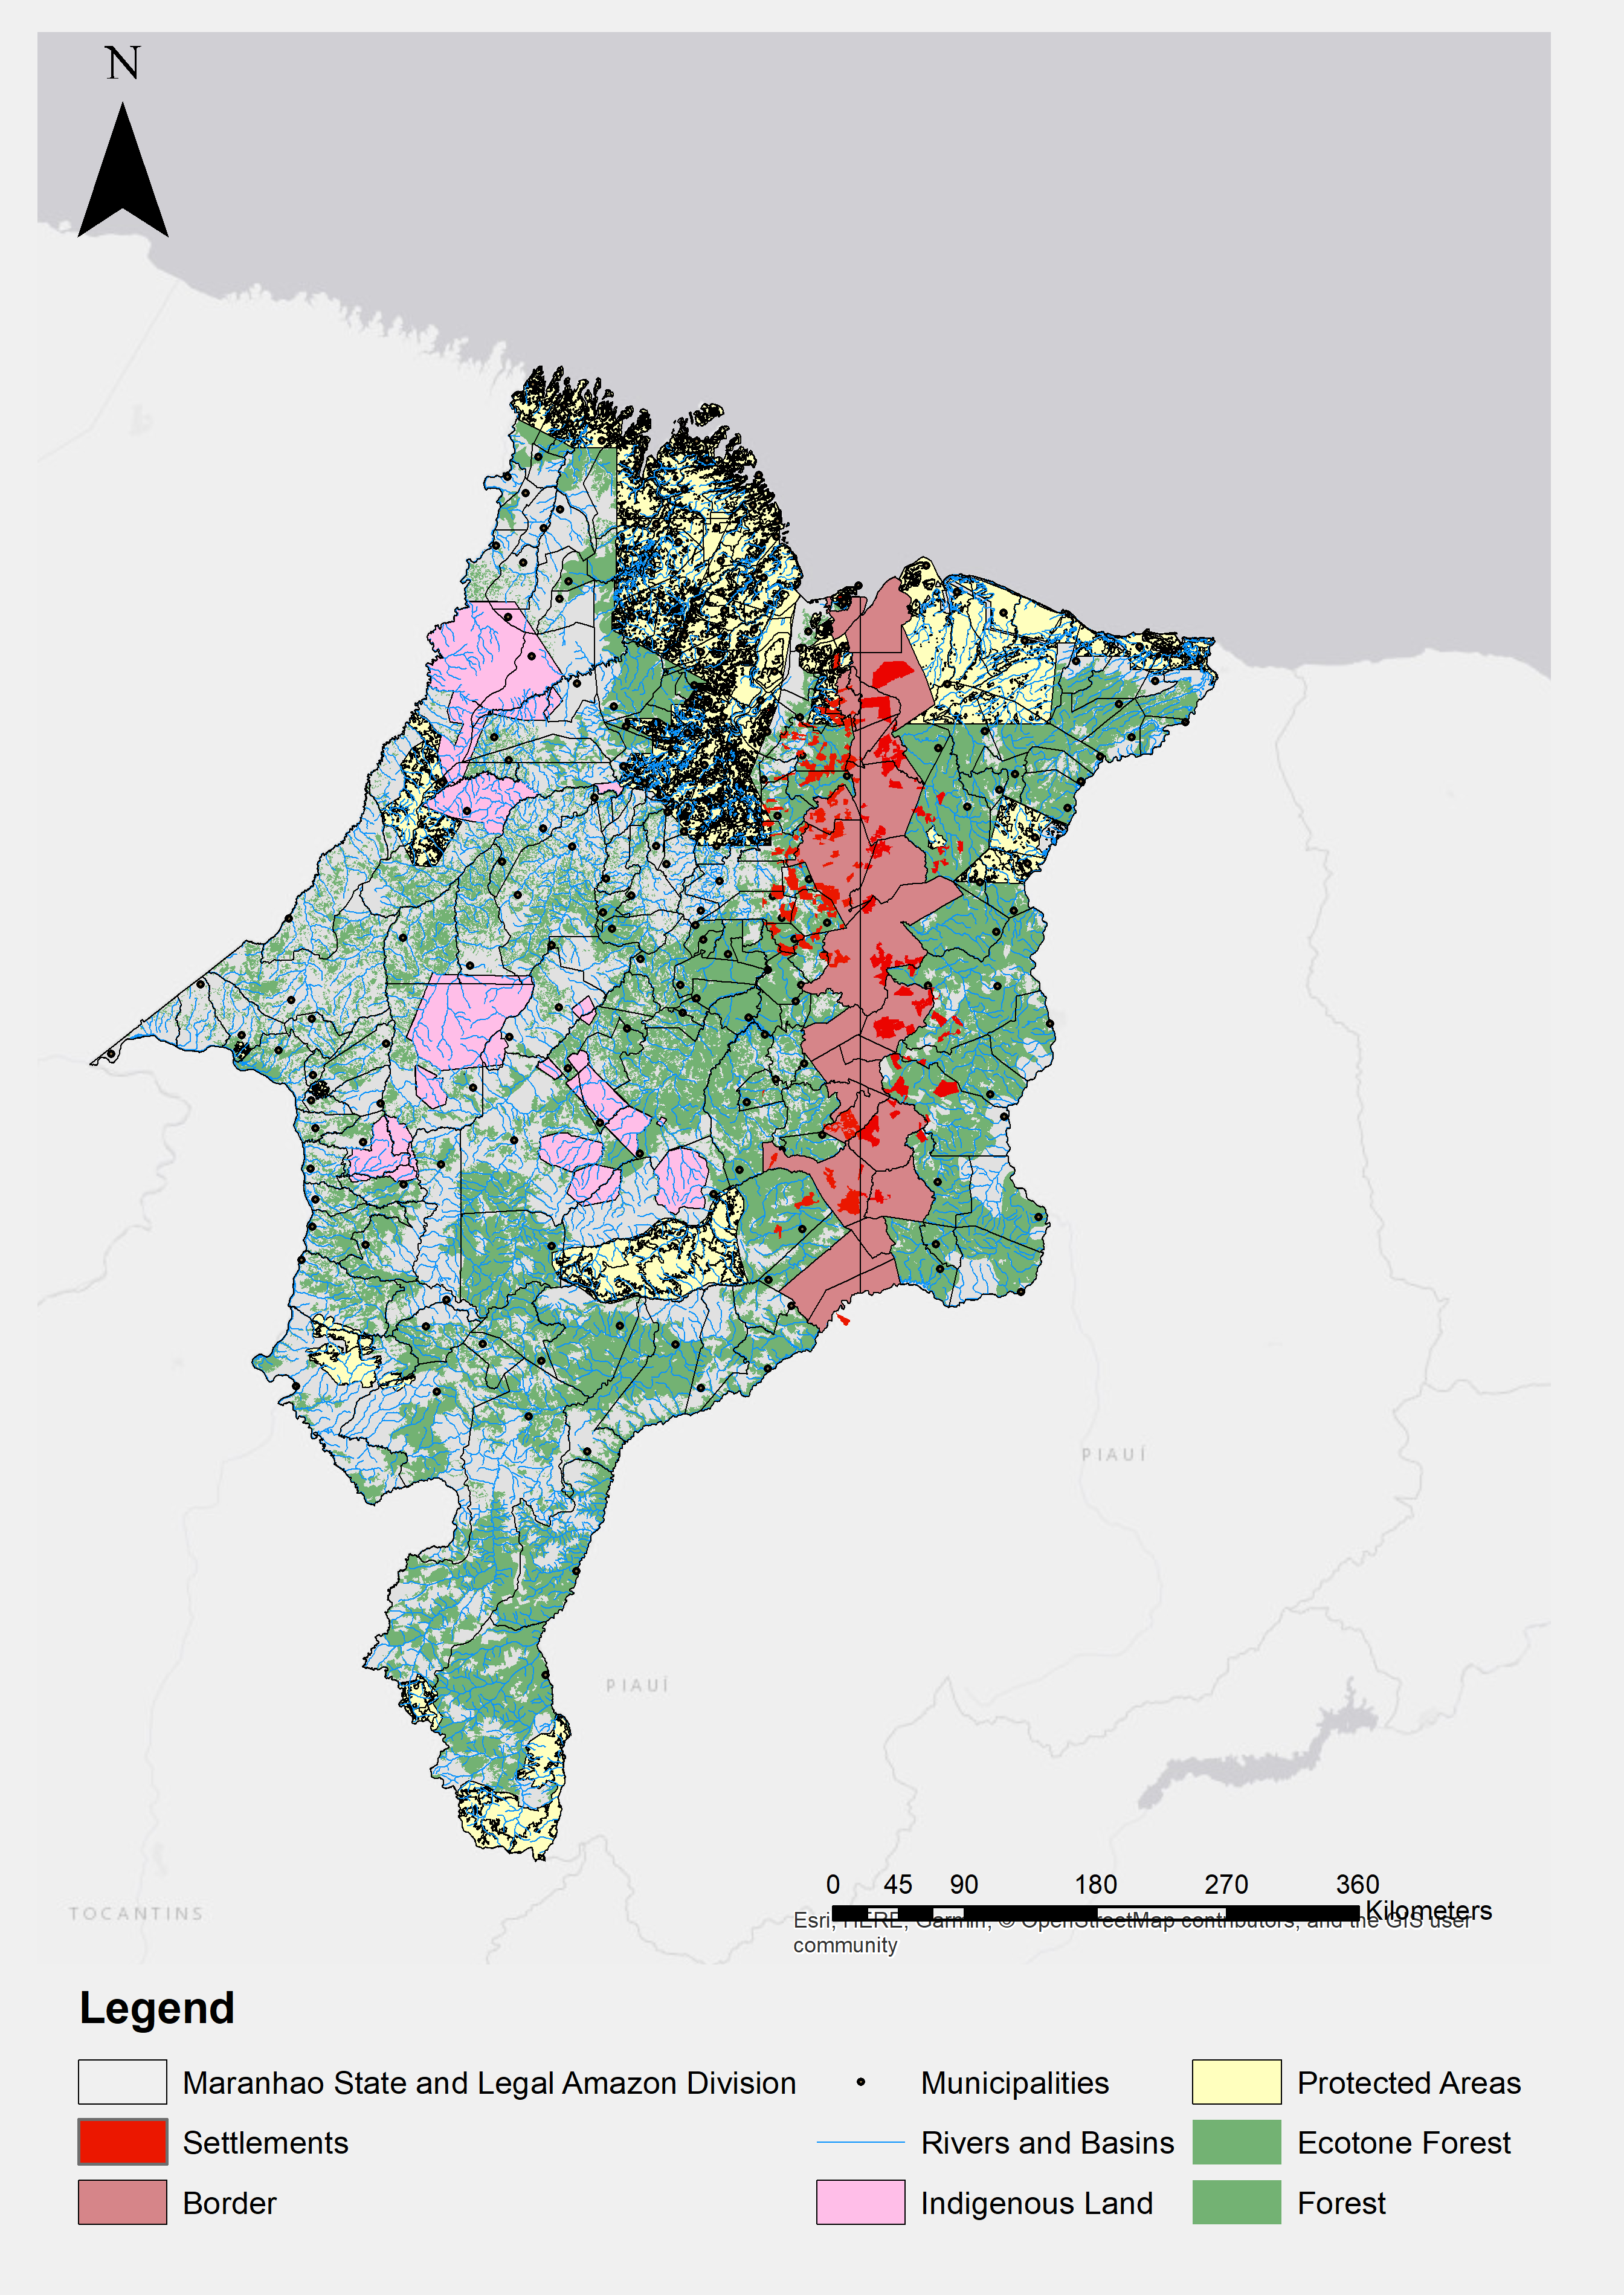
\includegraphics[width=1\textwidth, inner]{Chapter3/MaranhaoChapter3_Fig2.png}
\caption[Map of Maranhao including Settlements]{Map of Maranhao including Settlements. Source: \citep{MMMAwebsite,nugeo_2018}.}
\label{fig:delimitacaosett}
\end{figure}

The survival analysis in settlements follows the  Kaplan Meier fitter presented in Section \ref{resultssection1} and the Cox proportional hazard model with time dependent variable as demonstrated in Section \ref{resultssection2}. 

%KM fitter
The Kaplan Meier fitter shows that from the 37,532 pixels, in 2001, about 55\% of pixels had a chance of survival considering both vegetation indices. For 2010, the chance of survival decreased to the range of 5.8\% to 6.1\%. At the end of the studied period, the chance of survival for pixels within settlements were around 0.4\% and 0.6\% (see upper and bottom left graph from Figure \ref{fig:km-total-sett}). The median time of survival for the model was two years. This means that the half life of the sample pixels was around two years (the the 50th percentile). Sub-setting the survival curves by region, it's possible to identify that pixels within Legal Maranhão (LM) had a higher rate of survival comparing to pixels within Cerrado Maranhão (MA). The presence of clouds in this subset still shows that the chance of survival was higher in the Legal Maranhão (not shown). 

It was performed the Log Rank test \citep{Peto_1972} to check whether the two sub samples were originated from the same distribution and the differences from these survival curves are produced from other characteristics than the region. The results from the Log Rank test evidenced that these sub samples came from the same distribution which cannot reject the null hypothesis. However, given that the majority of the settlement pixels are deforested within two years, it was also applied the generalized Wilcoxon test, which can be also referred to Log Rank Weighted test, because it gives more weight to early deforestation than later deforestation, while Log Rank test gives equal weight to all deforestation process \citep{lee_wang_2003}. From the Log Rank Weighted test, at 5\% level, the two sub samples actually come from different distribution.

\begin{figure}[H]
  \centering
  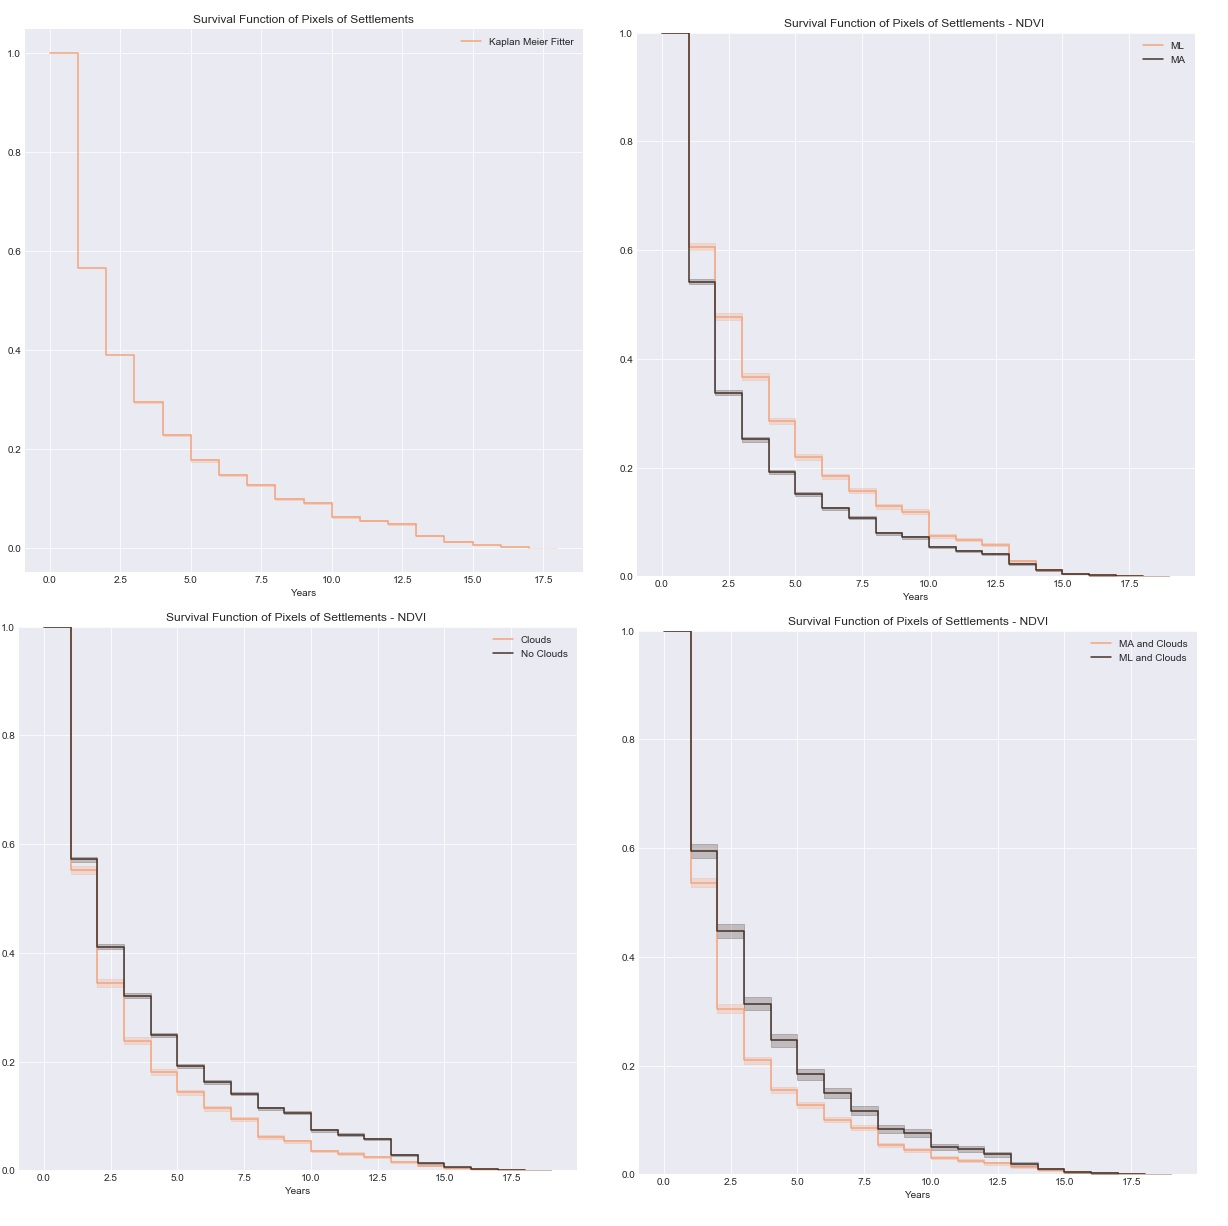
\includegraphics[width=1\textwidth]{KM_NDVI_sett_total.jpg}
\caption{Kaplan Meier Fitter for NDVI values in Settlements}
\label{fig:km-total-sett}
\end{figure}

%Cox time fitter
The results from the proportional hazard model is shown in Table \ref{tab:CPH_NDVI_sett}. The presence of clouds decreases hazard by 5\%. Elevation has a constant relative hazard. Distancing from municipalities centre decreases hazard by almost 27\%. Forested pixels within settlements and under the monitored policy area has a decreasing risk of being deforested comparing to non monitored areas. However, the presence of clouds in settlements located in the Legal Maranhão side increases the hazard by 4.2\%.


The extended Cox model presented in equation \ref{eq:8} is also applied to the settlements. The presence of clouds has no effect in the presence of the relative hazard. Distancing one unit from protected areas and mines increase by 12\% and 22\% the relative hazard, as can be seen from Table \ref{tab:CPH_NDVI_sett_time}. Municipalities centre are not significant in the model. The relative hazard decreases 80\% if the pixels are far from markets. Rivers and roads have no impact on relative hazard. The incidence of clouds in settlement pixels within the Legal Maranhão has no impact on the relative hazard. Increasing the level of rain decreases hazard by 0.01\%. Even though increasing the level of temperature increases the relative risk of a pixel being deforested, increasing the temperature in the Legal Maranhão decreases hazard by almost 3\%.

\begin{table}[H]
\footnotesize
\caption{Cox Proportional Hazard Model - Settlements}
\begin{tabularx}{\linewidth}{X YYYYY}
\hline
\hline
Variables	&	Regression Coefficient	&	Relative Hazards	&	Standard Errors	&	z score & Pr (>|z|) \\
\hline
Clouds	&	-0.052	&	0.950	&	0.014	&	-3.778	&	2E-04	***		\\
Pas	&	-0.011	&	0.989	&	0.045	&	-0.241	&	0.809			\\
Mining	&	-0.419	&	0.658	&	0.085	&	-4.933	&	8E-07	***		\\
Elevation	&	0.000	&	1.000	&	0.000	&	3.309	&	0.001	***		\\
Markets	&	0.026	&	1.027	&	0.029	&	0.903	&	0.366			\\
Municipalities	&	-0.306	&	0.737	&	0.084	&	-3.654	&	3E-04	***		\\
Rivers	&	1.431	&	4.183	&	0.345	&	4.148	&	3E-05	***		\\
Roads	&	0.234	&	1.264	&	0.139	&	1.685	&	0.092	.		\\
Lat	&	-0.154	&	0.857	&	0.018	&	-8.76	&	<	2E-16	***	\\
Lon	&	0.332	&	1.393	&	0.048	&	6.944	&	4E-12	***		\\
Region	&	-0.079	&	0.924	&	0.022	&	-3.525	&	4E-04	***		\\
Clouds*Region	&	0.041	&	1.042	&	0.021	&	1.995	&	0.046	*		\\
\hline
\hline
\multicolumn{6}{l}{Signs stand for '***' 0.001 '**' 0.01 '*' 0.05 '.' 0.1 and denote hazard ratios that are significantly}\\
\multicolumn{6}{l}{ different from 1 at 99\%, 95\% and 90\% confidence levels. The model contains controls for grouped year}\\
\multicolumn{6}{l}{periods. PAs stand for Protected Areas. Indigenous Lands and Conservational Units.}\\
\end{tabularx}%
\label{tab:CPH_NDVI_sett}%
\end{table}%

\begin{table}[H]
\footnotesize
\caption{Cox Proportional Hazard Model Time Dependent - Settlements}
\begin{tabularx}{\linewidth}{X YYYYY}
\hline
\hline
Variables	&	Regression Coefficient	&	Relative Hazards	&	Standard Errors	&	z score & Pr (>|z|) \\
\hline
Clouds	&	0.031	&	1.032	&	0.020	&	1.535	&	0.125		\\
PAs	&	0.116	&	1.123	&	0.066	&	1.766	&	0.077	.	\\
Mining	&	0.573	&	1.774	&	0.111	&	5.162	&	2E-07	***	\\
Elevation	&	0.000	&	1.000	&	0.000	&	2.376	&	0.018	*	\\
Markets	&	-0.218	&	0.804	&	0.042	&	-5.232	&	2E-07	***	\\
Municipalities	&	0.067	&	1.069	&	0.115	&	0.582	&	0.561		\\
Rivers	&	0.873 &	2.393 &	0.735 &	1.188 &	0.235	\\
Roads	&	-0.293	&	0.746	&	0.191	&	-1.53	&	0.126		\\
Lat &	-0.106	&	0.900	&	0.026	&	-4.074	&	5E-05	***	\\
Lon	&	0.016	&	1.016	&	0.057	&	0.288	&	0.773		\\
Region	&	0.573	&	1.773	&	0.111	&	5.162	&	2E-07	***	\\
Clouds*Region	&	-0.028	&	0.972	&	0.028	&	-0.99	&	0.322		\\
Neighbours	&	0.317	&	1.373	&	0.111	&	2.863	&	0.004	**	\\
Rainfall	&	-0.003	&	0.997	&	0.001	&	-5.331	&	1E-07	***	\\
Rainfall*Region	&	0.001	&	1.001	&	0.001	&	0.859	&	0.390		\\
Temperature	&	0.025	&	1.025	&	0.004	&	6.855	&	7E-12	***	\\
Temperature*Region	&	-0.021	&	0.979	&	0.004	&	-5.476	&	4E-08	***	\\
\hline
\hline
\multicolumn{6}{l}{Signs stand for '***' 0.001 '**' 0.01 '*' 0.05 '.' 0.1 and denote hazard ratios that are significantly }\\
\multicolumn{6}{l}{different from 1 at 99\%, 95\% and 90\% confidence levels. The model contains controls for grouped and }\\
\multicolumn{6}{l}{time-dependent year periods. PAs stand for Protected Areas. Indigenous Lands and Conservational Units.}\\
\end{tabularx}%
\label{tab:CPH_NDVI_sett_time}%
\end{table}%

\section{Discussion} 
\label{S:5}
Studies considering time event models for deforestation in Brazilian biome are not widely conducted and comparing the results becomes a complex task. The results presented in the previous section are then expanded and subtly generalised with prior studies on drivers of deforestation with different methodologies. The findings presented here can enhance and endorse the literature by this unique methodology in an ecotonic region of Brazil.

%Talking about the chance of survival being higher in the MA than LM and acknowledging that even with an environmental policy the pixels did not increase the chance of survival or decrease the rate of change (slowing the death). %Including cloud cover to the KM estimate.

%Politica Ineficiente - Regiao MA desmata menos que a ML
In the results, the non parametric analysis confirmed that the time of pixels surviving a process of deforestation is longer on the side of Cerrado Maranhão (MA) than on the side of Legal Maranhão (LM) which is under a surveillance policy. From the Kaplan Meier fitter, the chance of survival of pixels after one year of the implementation of the policy (2005) was almost 4 times higher in the MA region. In 2010, the chance of survival in the MA region was almost 5 times higher than in the LM region. Looking to the rate of change of survival percentage in MA region, it's possible to affirm that the rate of survival was about 40\% in 2001 declining to 20\% during 2002 to 2005. After this decline, the rate kept around 20\% until 2011 which there was a spike in the rate of change of survival pixels until 2016. For the LM region, the rate of change of survival rates oscillated more than in MA region. In 2001, the rate of change was about 50\% and started decreasing to about 33\% at the end of 2006. The rate of change of survival pixels had a peak in 2007 and decreased between 2008 and 2012. After this period, the rate of which the pixels survived from one year to another increased until the end of the studied period. These rates indicate that the rate of pixels surviving was decreasing much faster in the LM side than in the MA side. From the findings, it suggests that the environmental policy was undermined in the Legal Maranhão (LM) area. 

The situation is similar when observing the presence of cloudy pixels in these regions. The probability of a clouded pixel surviving in the Cerrado Maranhão (MA) is at least 4 times higher in 2005 and, in 2010, 9 times higher than in the Legal Maranhão (LM). These results reveal that the environmental policy taking place in the LM region did not increased the chance of pixel survival in that particular region. We believe that the presence of clouded pixels influenced the effectiveness of the policy. 

Knowing that many studies considered other drivers of deforestation than clouds, the outcome was expanded to the inclusion of other covariates or risk factors. 
%Explaining Cox model given a special treatment to Pas, roads and clouds region.
%Um olhar sobre os Risk factors
The results from Tables \ref{tab:CPH_NDVI_MA_ML}, \ref{tab:CPH_NDVI_MA}, \ref{tab:CPH_NDVI_ML}  reflect the chance of a pixel surviving under the combination of these two areas (Region), Cerrado Maranhão (MA) and, Legal Maranhão (LM), respectively. The first risk analysed is the persistent presence of clouds. The Region results show that clouds has a positive effect on the relative hazard. When interacted with the satellite monitored area the effect is not significant even though the existence of forested pixels within the Legal Maranhão increases the chance of being cleared. For the Cerrado Maranhão (MA), this risk factor decreases the chance of a pixel being deforested, for example, rainy periods were a positive aspect to reduce deforestation. For the LM region, the results show a non significant result. 

Adding time dependent risk factors and controls, the results from the Region illustrate the scenario that clouds increase the risk of a pixel being deforested. Clouded pixels has a higher chance of being deforested but this effect does not seem to be significant when conditioning on the environmentally monitored area. We include in the analysis other aspects that might indicate rainy periods and, when conditioned on the Legal Maranhão (LM) implicate cloud cover effect. In LM side, intensified rainfall increases hazard and high levels of temperature decreases it. This outcome provides a possible explanation that the survival of forested pixels was higher with clear upper atmosphere.

%PAs as instrument to curb deforestation - fuel as well
In addition, another important aspect is shown from the results. Protected areas, which include conservation units and indigenous land, seem to be a positive risk factor for deforestation when looking to the Region. Forested pixels close to protected areas had a higher chance of being deforested comparing to forested pixels far from these special zones. From the proportional hazard model results for the Region, this policy had a negative effect on increasing the chance of forest survival. With the inclusion of time dependent variables and further controls, it's possible to observe that the pattern persists for the Legal Maranhão (LM) and Cerrado Maranhão (MA) as well. 

It is documented that the Maranhão State has less than 20\% of its whole territory under any sort of environmental protection \citep{SPINELLI_2016}. Counting the Cerrado and ecotonic areas only, this percentage drops to 12.5\%. In this sense, we understand that one possibility is that PAs, specially conservational units, are established in response to previous deforestation pressure which is then displaced to neighbouring areas just outside the PAs and is therefore capturing the presence of active groups of loggers in a closed area. The second possible explanation regards to the fact that there are potentially limited public monitoring and enforcement in this transitional forest area, specially in the not satellite monitored side.\footnote{These possibilities were observed in the Conservational Unit of \textit{Morros Garapenses} on the Cerrado Maranhão (MA) side. The unit was created in 2008 with the aim to protect the diversity of representative regional ecosystems that functioned as habitat for native and migratory species, as well as wildlife refuges from areas already devastated by human activities \citep{isa_2018}.}  

%Roads increase pixels hazard 
The findings indicate roads distance as a risk factor for the survival analysis. Roads in Cerrado Maranhão (MA) increase the chance of deforestation to occur. Forested pixels far from roads had a higher rate of survival. Roads as a driver of deforestation is also discussed in the literature \citep{CROPPER2, CROPPER1, PFAFF3, BAYNARD} which uphold our findings. Interestingly, roads is not significant in the monitored area when controlling for time and space. This aspect might relate to several actions implemented in the Legal Amazon to detain deforestation through roads surveillance which refrained deforestation process along major roads.\footnote{'Arc of Fire' special force was created in 2007 by the federal government to combat the increased pace of deforestation in the Amazon recorded from INPE results \citep{PF_arcodofogo,inpe-deter_2018}.} 

%Markets and munics
Looking to the time dependent models, markets and municipalities centre are insignificant in the Region but these risk factors show different effects in the MA and LM sides. For both areas, forests distant from municipalities centre have a higher chance of survival. This might reveal that urbanisation accounted for deforestation in these areas. On the other hand, distancing from markets increased the probability of a pixel being deforested. It comes to the knowledge that great part of the environmental and fiscalization police are located close to markets, specially those dealing with logger, grains and cereals products, so forests close to the municipalities had more visibility to be inspected and accessed and then preserved \citep{rural_2018}.

We turn our discussion to our time dependent controls and risk factors. Neighbours, rainfall and temperature were included in the model to account for spatial and temporal changes. From the Region table, rainfall and temperature decreased the risk of a pixels being deforested while neighbouring forested pixels increased the potential risk. As mentioned above, temperature and rainfall conditioning on the environmentally controlled area confirm that pixels had a higher chance of survival during dry season. This reflects the prominent changing behaviour experienced in the Legal Maranhão (LM) comparing to the non Legal side. The latter has a different dynamic when we observed temperature and rainfall risks. According to the results, in the Cerrado Maranhão (MA) happened the opposite situation with high levels of rainfall decreasing the risk of a forested pixel being cleared. The interpretation relies possibly in the fact that clear cutting process became costly when intensive rain occurred. When temperature increased, the risk of deforestation also increased, differing from the Legal Maranhão (LM) findings.

%Explaining Cox model time dependent given a special treatment to neighbours
%Pressao das florestas vizinhas eh um fator acelerador pra morte dos pixels
%The inclusion of neighbouring pixels at different time periods allowed the Cox Proportional model to vary over time and to control for spatial and temporal heterogeneity that could arise from the analysis. From Table \ref{tab:CPH_NDVI_MA_ML_time}, forested pixels covered by clouds over the period was not significant. Protected areas are a benefit to the survival of forests. Overall, distancing from mines, markets and municipalities centre increase the risk of the endurance of forested pixels. Particularly, great part of these sign effects is due to the Cerrado Maranhão (MA). As stated previously, roads are considered a great risk for forest in that region. Once again, forested pixels covered by clouds in the surveillance area has a higher chance of being deforested than in the not monitored area. Finally, having forested pixels nearby increases the chance of being deforested which is assimilating the anthropic pressure on the environment.

In an attempt to check the validity of the results, we conducted the same approach on i) areas immediately outside the studied area with a threshold of 0.2 decimal degrees and ii) in settlements areas within the complete region. 

The non parametric results demonstrate that the chance of survival is higher for pixels inside the satellite monitored area and unexpectedly in the presence of clouds. This configures that the effect of the surveillance policy is substantiated when the distance increases from the artificial line. 

For the proportional hazard model, clouds decreased the risk of pixel being deforested in the buffer zone. It was addressed that pixels within the Legal Maranhão buffer had a higher rate of survival comparing to pixels located in the Cerrado Maranhão buffer but when these pixels were conditioning on cloud persistence the risk of deforestation increased. For this particular zone, protected areas increased the chance of a forest nearby to survive. In the extended model, protected areas still increase the chance of survival of nearby forested pixels and, pixels located in the monitored policy area had an extremely higher chance of survival (99\%) which agrees with the non parametric results. When dividing the sample in the two areas, the effect of the time dependent variables and our interest variables become insignificant for both sub samples. We understand that increasing the distancing area, local characteristics tend to recede. 

Considering that settlements are not regulated by municipalities and, are not directly punished for deforestation from the surveillance program. It is feasible to credit that these plots are not influenced by local institutions and environmental policies. From the Kaplan Meier fitter, it shows a different path from what have been seen for the studied area. Figure \ref{fig:km-total-sett} shows that forested pixels had a higher chance of survival in the Legal Maranhão region than in the Cerrado Maranhão. Categorically, the rate of survival was higher for settlements areas within Legal Maranhão which arises the assumption that even not supervised directly by the environmental policy, the settlements preserved more forest than public and private forested lands. 

% Falar que os assentamentos demoram mais a desmatar comparando com o ML e a nivel de assentamentos por regiao, MA desmata mais rapido que o ML - Nuvens nao influencia para os assentamentos 
%Rivers sao sinal de survival para os pixels

Including the same risk factors and time dependent controls, the results reveal that forested pixels covered by clouds had no effect within settlements. Also, forests in remote settlements had a significant higher chance of survival when comparing to settlements close to markets. It shows that settlements close to market and urbanised areas usually are the first plots to be allocated, during the 50's, and are considered more developed \citep[p.~12]{alencar_2016}. Furthermore, these settlements were created several decades ago and the pressure on remaining forests is higher than on the new remote allocated settlements. Clouded forested pixels in settlements within the Legal Maranhão is not significant and, the increasing level of temperature decreases the risk of a pixel being deforested which is similar to the results from the Legal Maranhão (LM) side. However, rainfall and temperature follow what was observed in the Cerrado Maranhão (MA).

%(1) if the probability of deforestation was higher in the region not controlled by a specific environmental policy
Thanks to the results found in this study, we can outline possible responses to our discussion. Considering the Region and sub sample areas, the probability of deforestation was relative higher in the region controlled by the environmental policy. This outcome contradicts our assumption that environmental policy could refrain further deforestation. However, when we performed robustness checks in different settings, we could see that the rate of survival was higher in areas within the environmental policy. What brings into our attention is the fact that areas in the Legal Maranhao close to the artificial line had a lower rate of forest survival and, distancing from the artificial line the chance of survival increased comparing to distanced areas in the Cerrado Maranhao. Even though the median time did not change for most of the specification and robustness checks, the rate was inversely related to the distance of the Legal Amazon limit. We further document that areas inside the differentiated environmental policy but not subject to it, i.e. settlements, showed a higher rate of survival when comparing to the other side of the analysis. Notably, many of these settlements are located very close to the artificial line however it did not affected the settlers behaviour. Studies confer to these settlements the responsibility of deforestation in the past decades. However, our results prove that settlements appear to let their forest survive for a longer time than non settlements areas. We can see that the environmental policy was undermined in the ecological tension zone of Maranhao. 

%(2) what factors may be influencing the risk of the two regions to be deforested? And, 
We show that clouds persistence, protected areas and, roads are a great risk to the survival of forests. Not surprisingly, protected areas reflect the action of past deforestation and then, the pressure on these special zones is transitioned to their borders. The presence of roads indicates infrastructure expansion and is usually considered a proximate driver \citep{LAMBIN1,LAMBIN2}. Our findings corroborate to the existent deforestation literature. 

Based on a recent study (Chapter 2), we tried to confirm that much of deforestation shifted from dry to rainy season. Clouds persistence increases the risk of deforestation in the Region. We only see this persistence for the Legal Maranhao side (Table \ref{tab:CPH_NDVI_ML_time}). Since the areas are identical in several aspects (see Table \ref{tab:summaryMALM}), the net effect corresponds to the presence of clouds. We interacted the climatic controls to reassure this assumption and we were able to discern that increased level of rainfall and temperatures falling signified rainy season. 

%(3) if changing behaviour undermined the effect of the policy.
Finally, with the buffer zone and settlements analysis, it is likely that the environmental policy could not detain deforestation during the last two decades in the ecotonic region of Maranhão. According to the results, the forests inside the surveillance area had a lower probability of survival comparing to the area not covered by the policy. The presence of clouds along with climatic variables was an active barrier to the legal compliance and, since the studied area has no systematic differences, we can agree on the lack of effectiveness due to cloud barrier. Since these barrier indicate different form of seasonality, the probability of a pixel being deforested in the rainy season is higher comparing to dry season which in turn evidence the behaviour change. We deduce that our results justify the undermining effect of the environmental policy caused by the changing behaviour and the presence of the artificial line. 

\section{Conclusions}
\label{S:6}

In this study, we employed a survival analysis approach to detect the probability of occurring deforestation in the transitional forest of Amazon and Cerrado biomes. The technique applied used data derived from satellite images combined to several covariates. It was created an algorithm to capture Vegetation Indices changes over time in order to create a list of the time of a pixel was disturbed (deforested) as a response variable. An artificial line, called the Legal Amazon line was used to divide the analysis in terms of two regions, Legal Maranhão (LM) and Maranhão (MA), according to their differing treatment in deforestation protection.  

In the results, we conclude that protected areas and roads are a great risk to the survival of forests. Protected areas reflect the action of past deforestation and then, the pressure on these special zones is transitioned to their borders. Roads indicate infrastructure expansion and is usually considered a proximate drivers. Our findings explain that forests close to roads has a higher chance of being cleared. Mainly, forested pixels covered by clouds in the surveillance area has a higher chance of being deforested than in the not monitored area. Having forested pixels nearby increases the chance of being deforested which is assimilating the anthropic pressure on the environment. Finally, rainfall and temperature also affects the hazard. For the environmentally regulated region, intensive showers and lower temperatures increase the probability of a forested pixel being deforested. For the non regulated side, rainfall and lower temperature decreases the aforementioned probability.

We acknowledge a number of limitations to the resulted analysis. Firstly, the model implicitly assumes that in the first year of the study all pixels are fully occupied by forest, which in reality might not be true. It is also possible that the spatial distribution of the vegetation indices may exhibit dynamic behaviour over time, so that a potential area may or may not be sparsely vegetated for a certain period (e.g., during sampling) due to progressive succession of forest or attack of pests and diseases which is not captured by the vegetation indices. Secondly, the study was based on coarse image resolution which could neglect local changes (< 250m) in the sample area. Thirdly, our results may not be generalised to other areas, such as dense tropical forests and sparse open fields. In addition, we only considered for the analysis covariates existent before or from 2000, which excluded roads, protected areas, indigenous land, markets, municipalities centre, and, mining/mineral resources created or discovered after 2000. Finally, we understand that the models were derived from NDVI values which tend to be the second best choice of vegetation index comparing to EVI values for ecotone forests \citep{ratana_huete_ferreira_2005,bayma_sano_2015,didan_munoz_2015}.

\let\cleardoublepage\clearpage
\begin{appendices} \label{appendix}
\renewcommand{\thechapter}{A.\arabic{chapter}}
%!TEX root = ../chapter3.tex
% ******************************* Thesis Appendix A ****************************

\chapter{}

\begin{sidewaystable}
\begin{figure}[H]
  \centering
  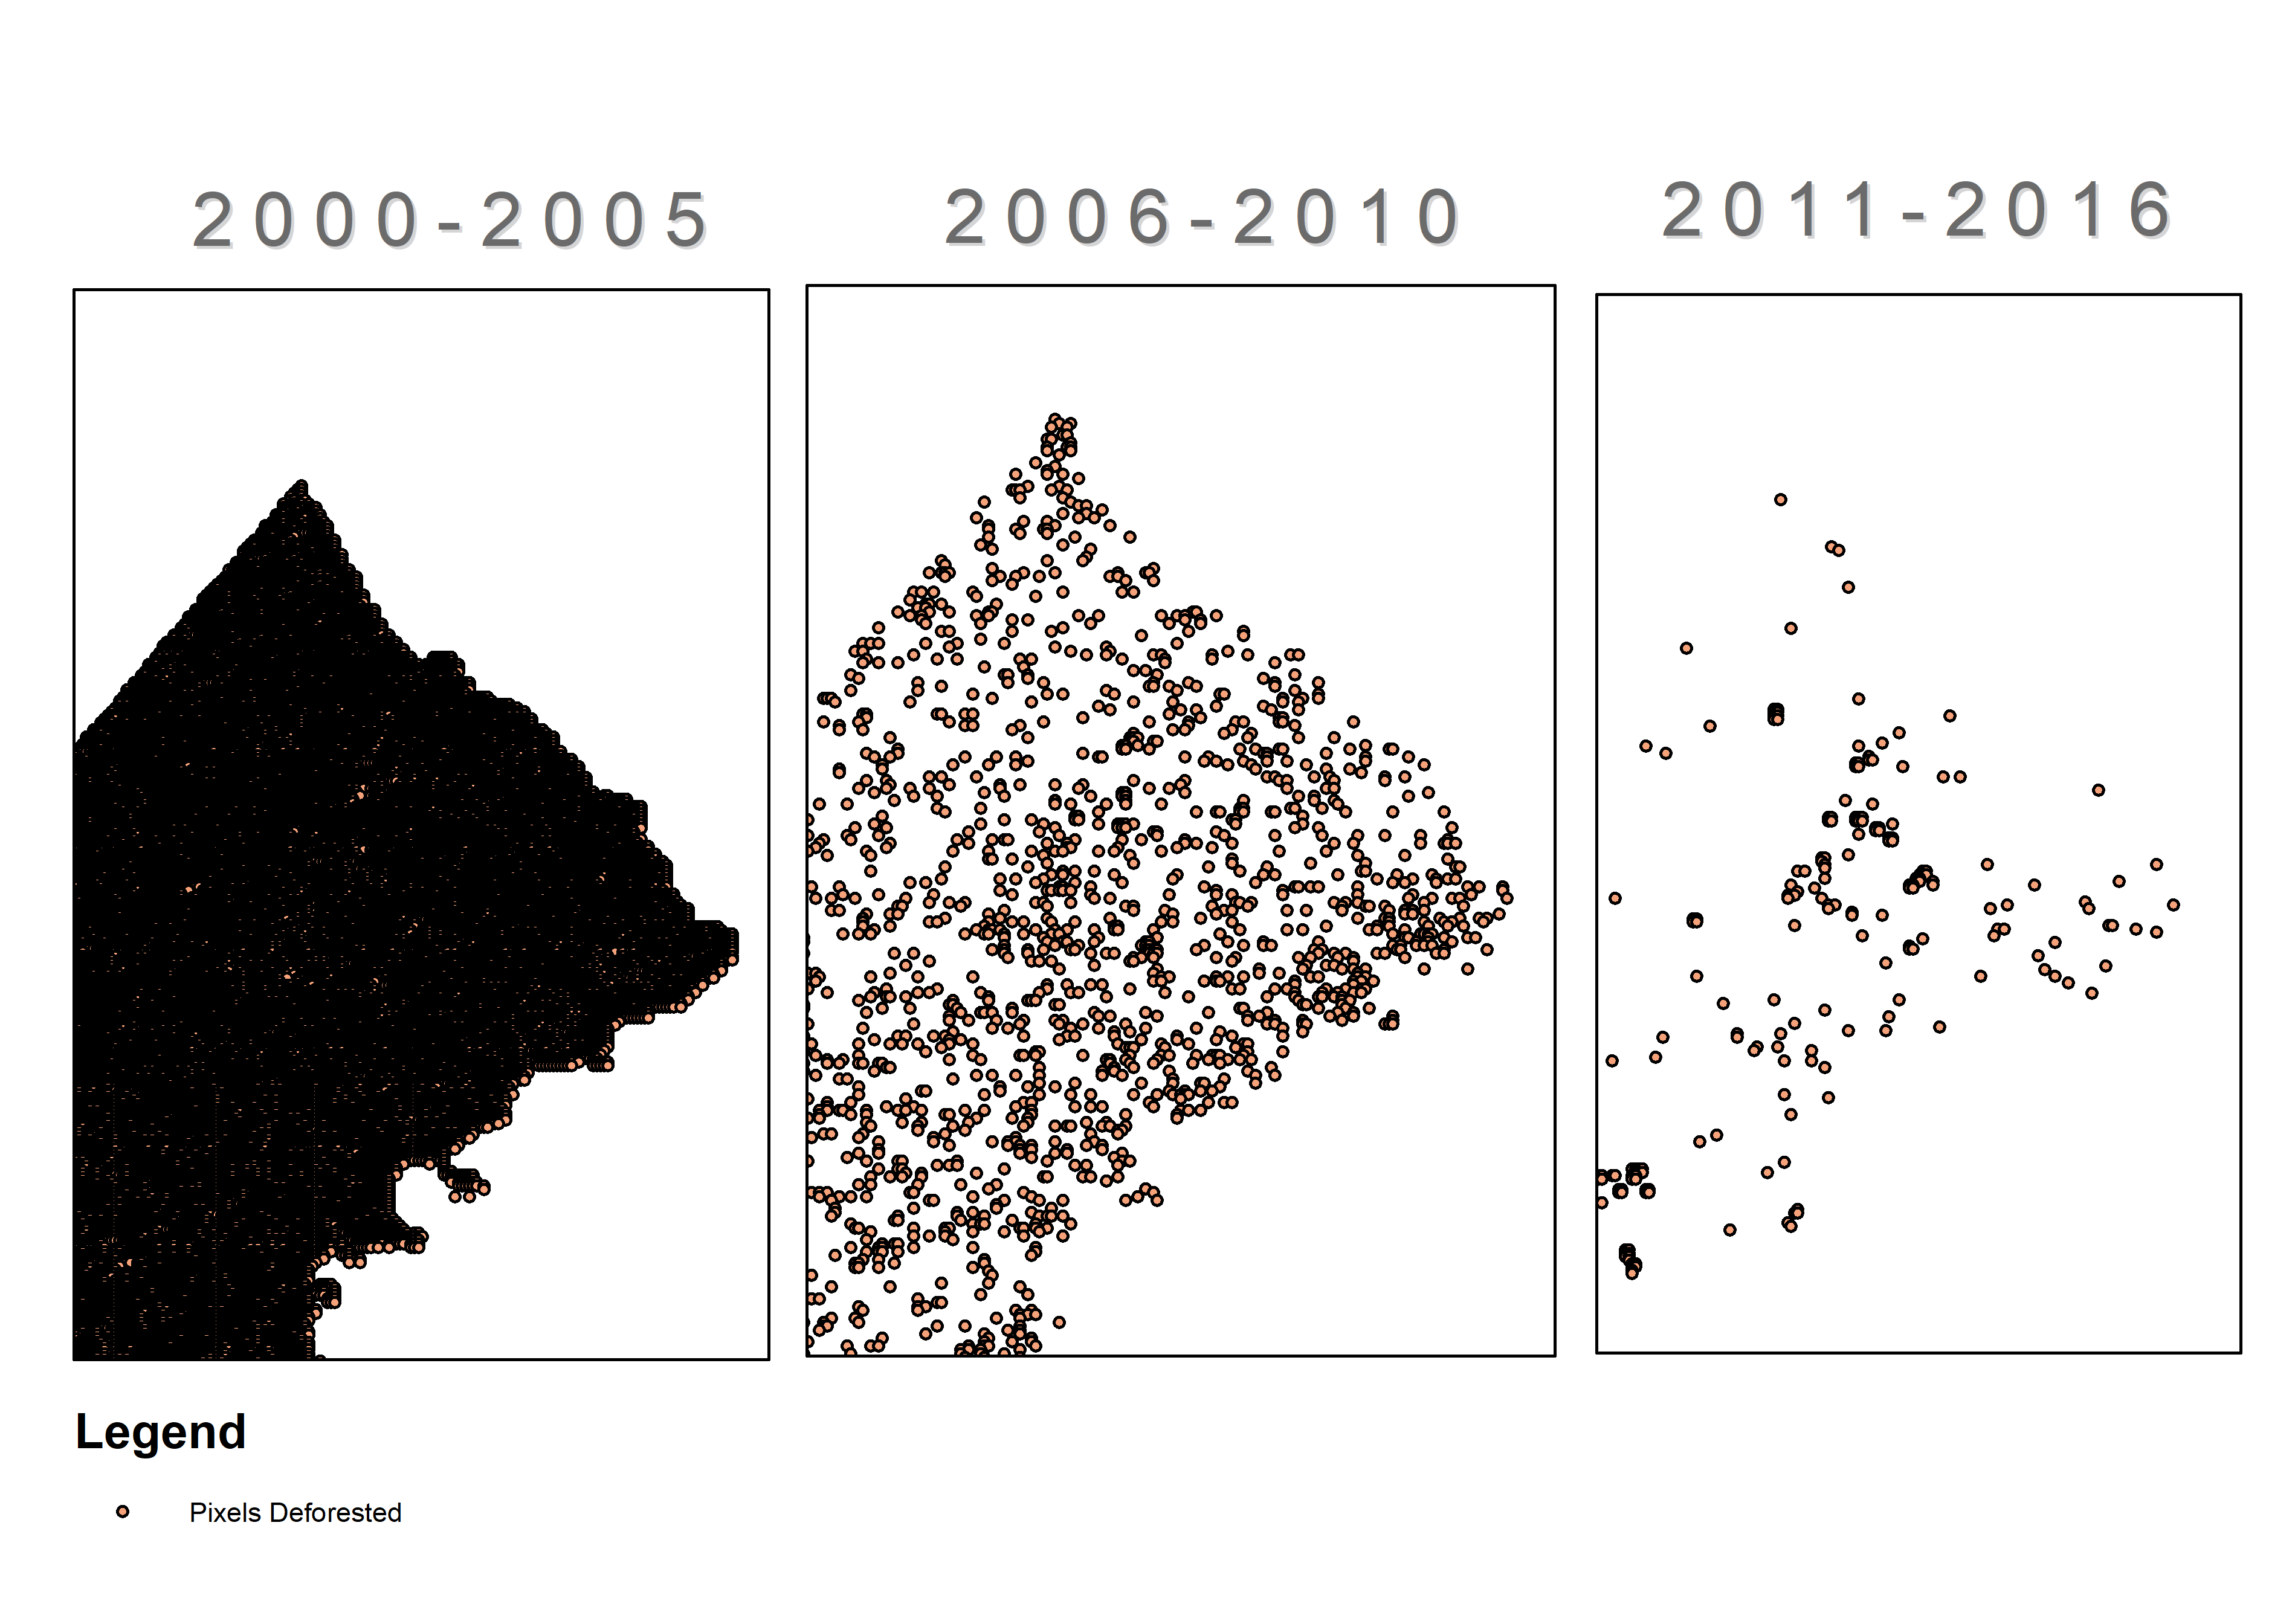
\includegraphics[width=0.85\textwidth]{Chapter3/ML_pixels_death.png}
\caption[Remaining Pixels in Legal Maranhão side]{Remaining Pixels in Legal Maranhão side for three different year periods. Pixels are only counted once. Area was randomly chosen.}
\label{fig:remainingLM}
\end{figure}
\end{sidewaystable}

\begin{sidewaystable}
\begin{figure}[H]
  \centering
  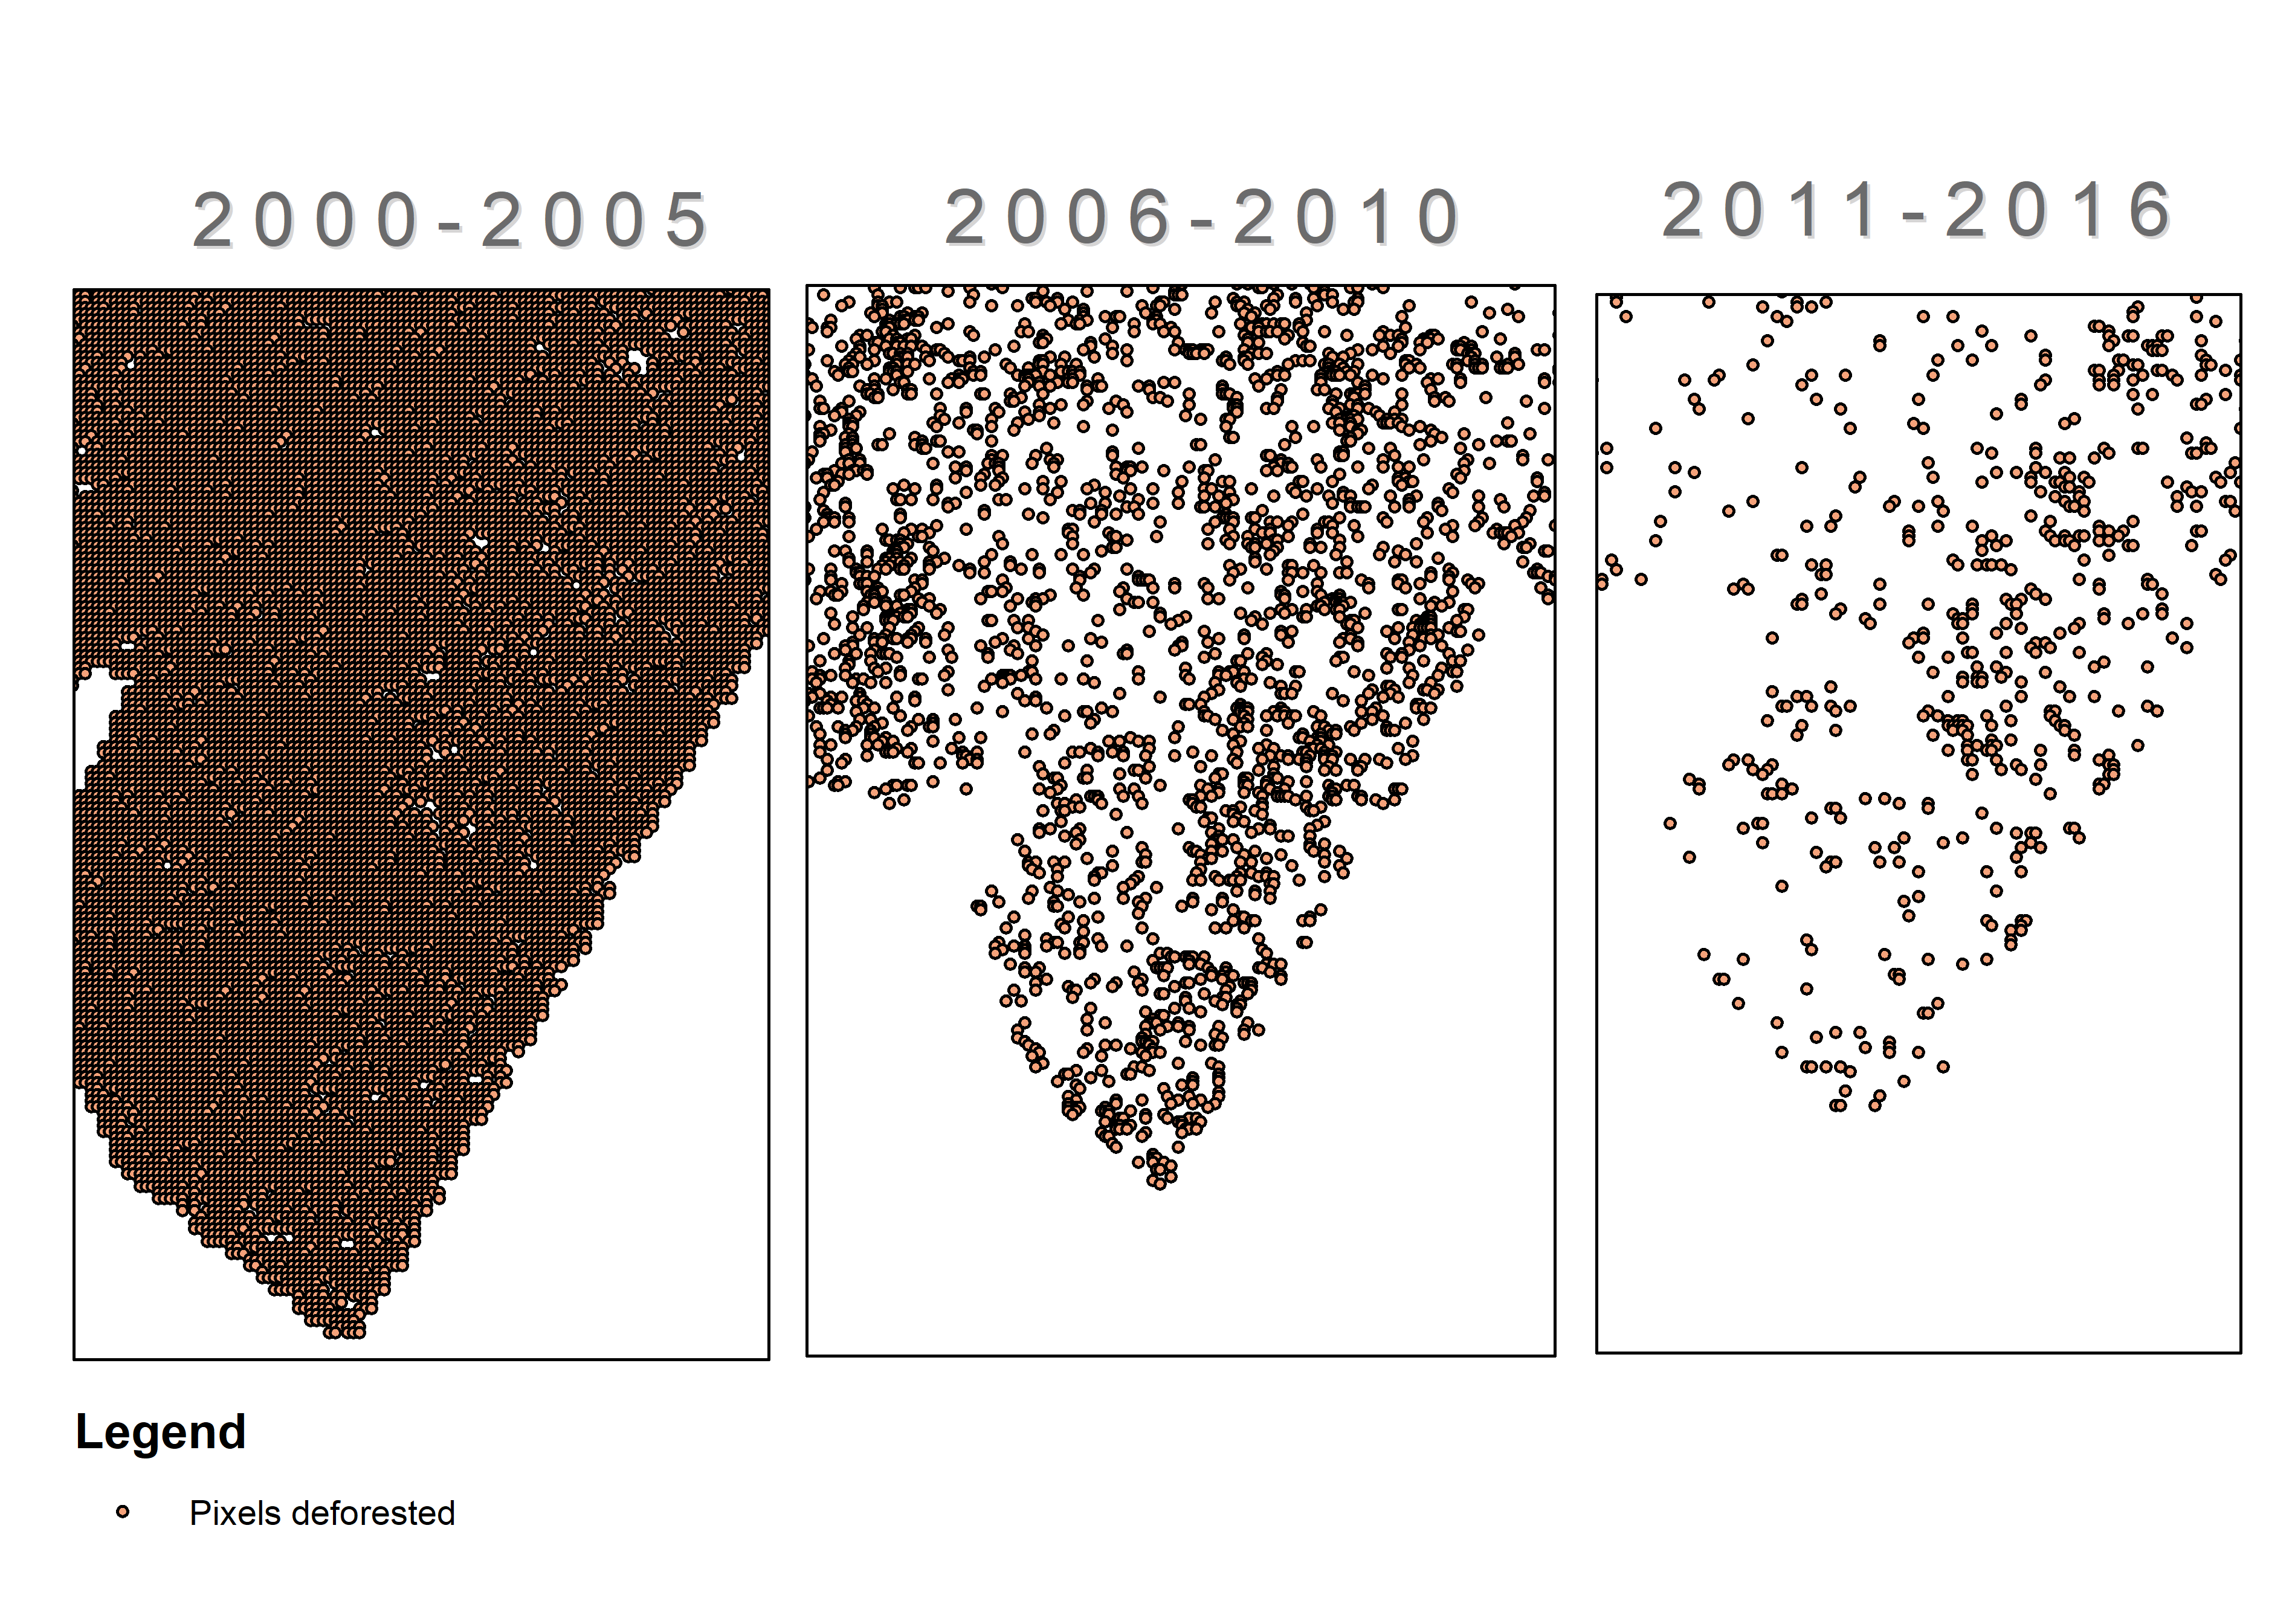
\includegraphics[width=0.85\textwidth]{Chapter3/MA_pixels_death.png}
\caption[Remaining Pixels in Cerrado Maranhão side]{Remaining Pixels in Cerrado Maranhão side for three different year periods. Pixels are only counted once. Area was randomly chosen.}
\label{fig:remainingMA}
\end{figure}
\end{sidewaystable}

\begin{sidewaystable}
\begin{figure}[H]
  \centering
  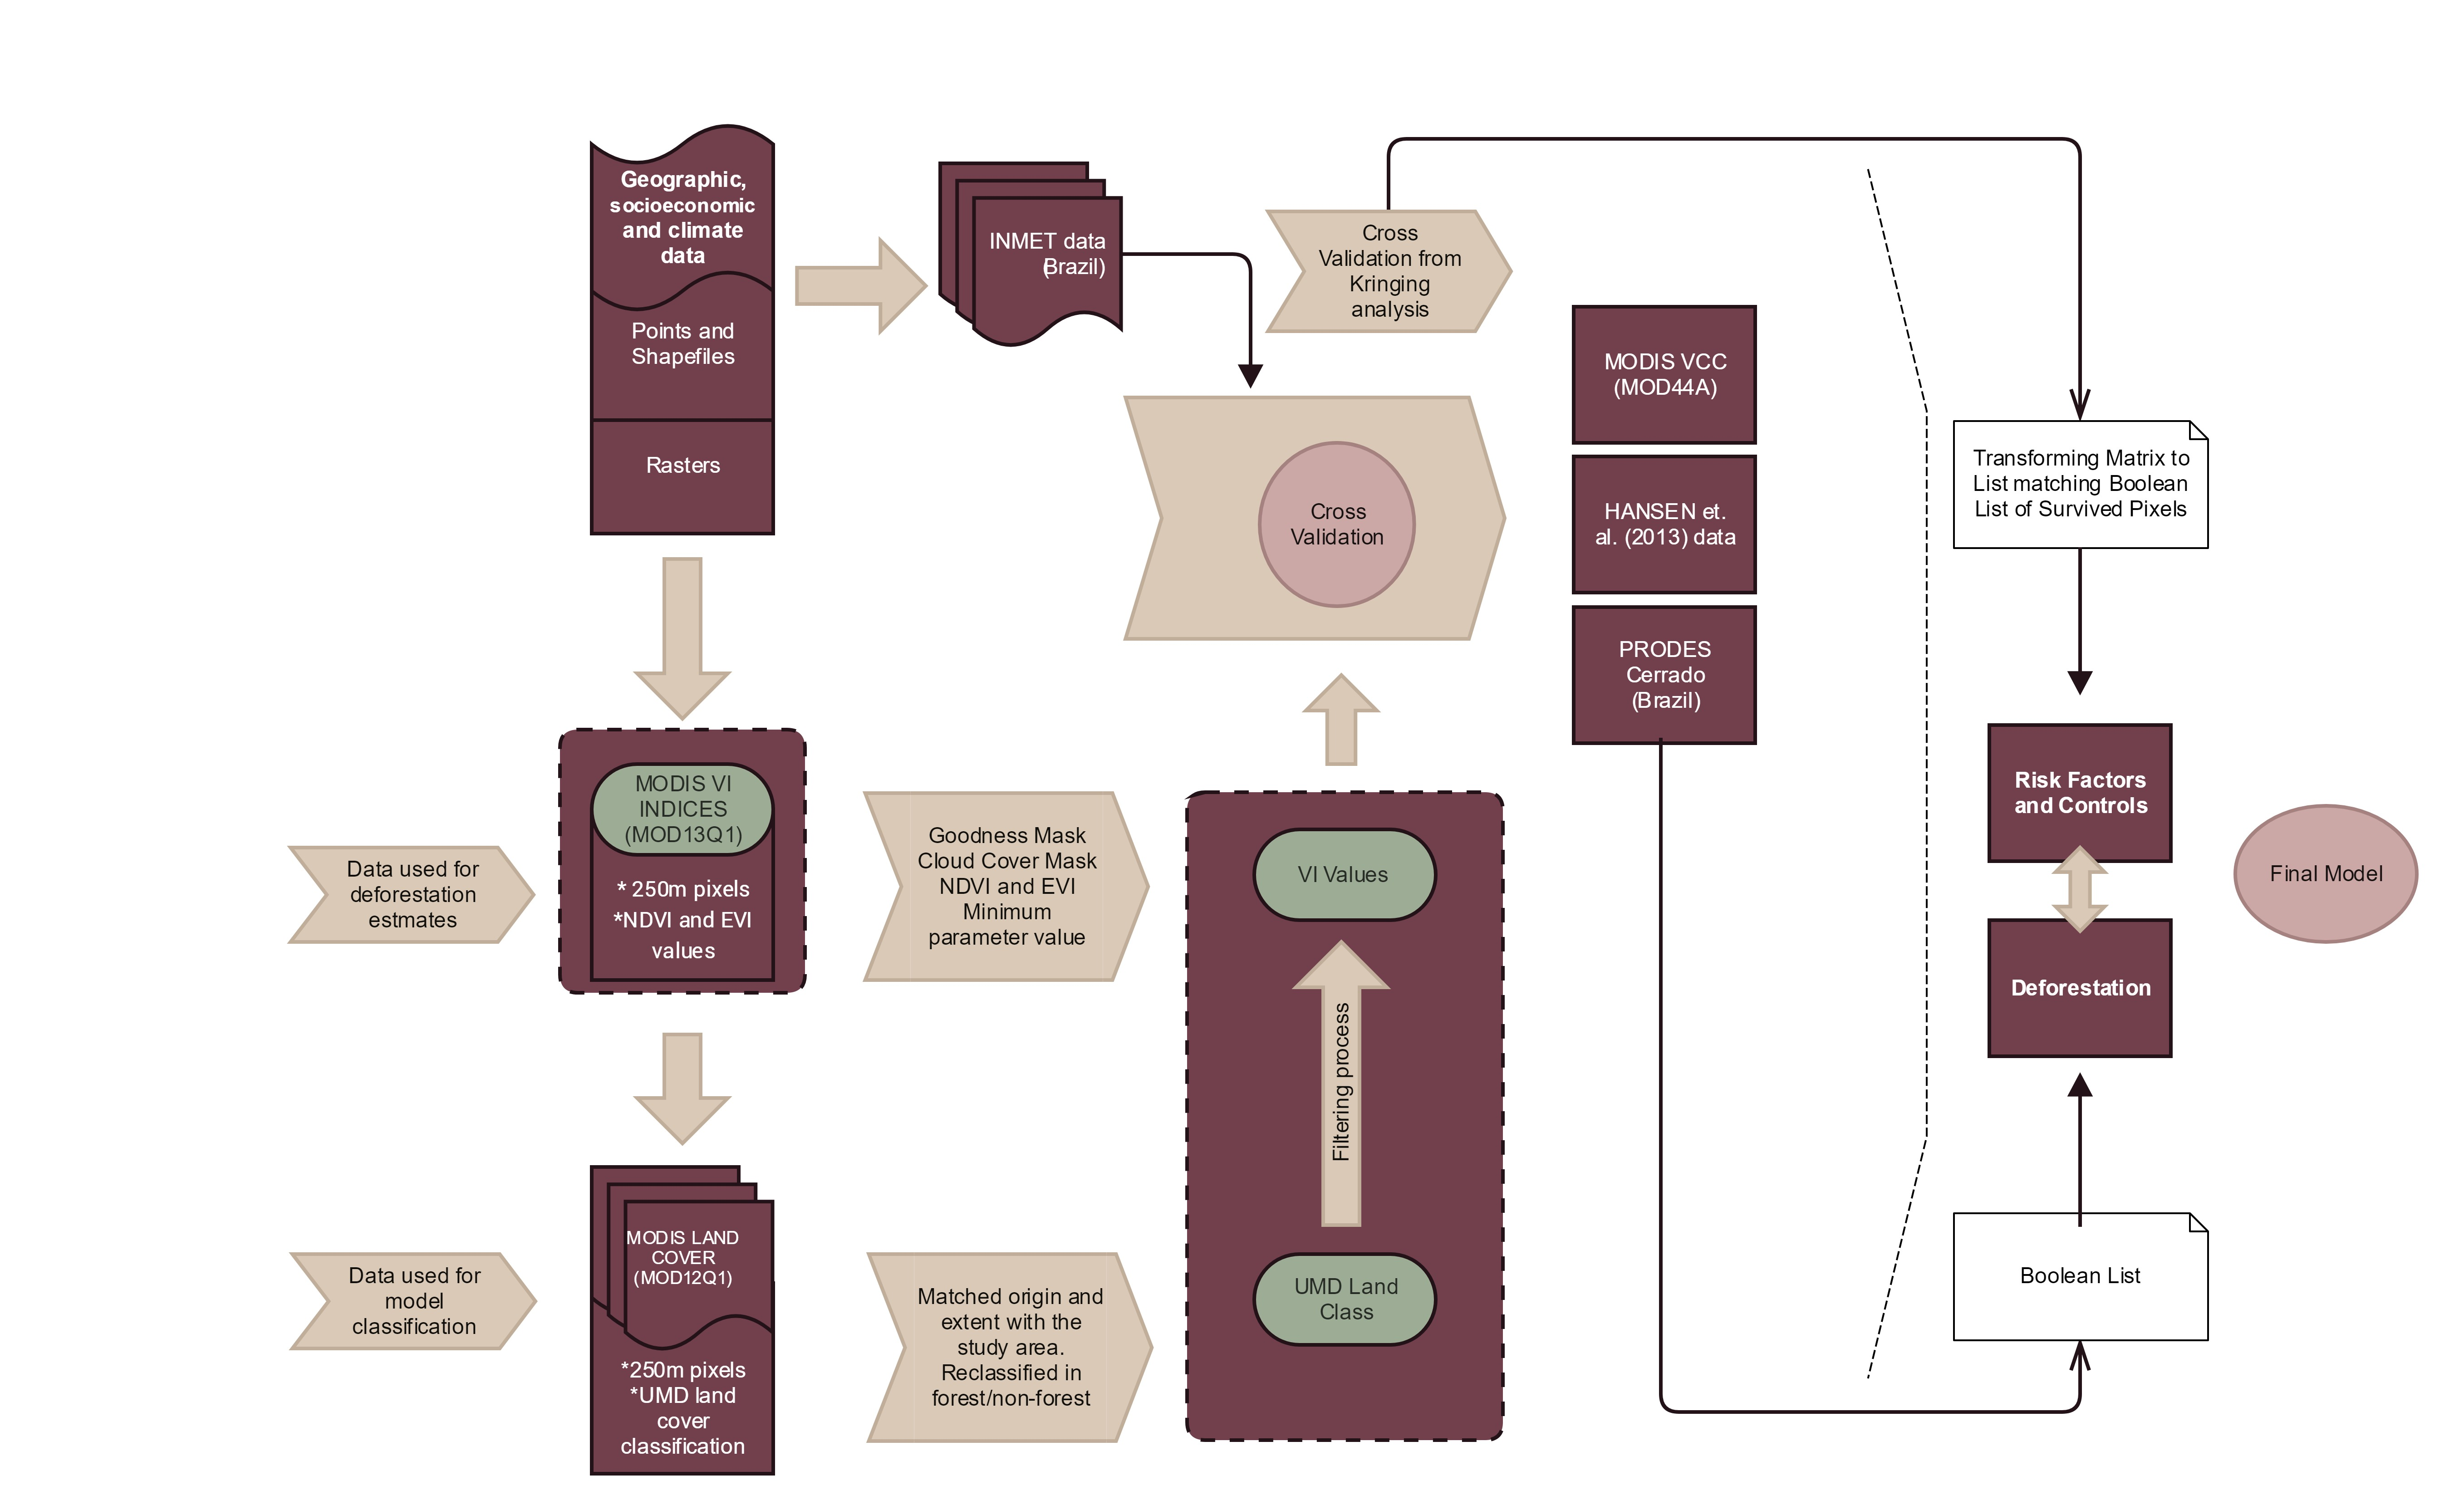
\includegraphics[width=9\textwidth]{method.jpg}
\caption[Flowchart of method applied to data]{Flowchart of method applied to data. Moving from left to right indicates increasing levels of data processing during the study.}
\label{fig:method}
\end{figure}
\end{sidewaystable}

\begin{table}[H]
\footnotesize
\caption{Model Selection and Validation}
\begin{tabularx}{\linewidth}{X CCCC}
\hline
\hline
Models	& Concordance index & Std Deviation &	K-fold (k=3)	&	Std Deviation \\
\hline
NDVI MA	& 0.767 & 0.001 &	0.30	&	0.0004 \\
NDVI ML	& 0.691 & 0.001	& 0.69	&	0.0008 \\
NDVI Region & 0.755 & 0.001	&	0.03	&	0.0004 \\
EVI MA	& 0.735 & 0.001	& 0.39	&	0.0011 \\
EVI ML & 0.691 & 0.001	&	0.69	&	0.0008 \\
EVI Region & 0.732 & 0.001	&	0.08	&	0.0008 \\
NDVI Sett MA & 0.780 & 0.003 &	0.77	&	0.0040 \\
NDVI Sett ML & 0.798 & 0.003 &	0.79	&	0.0019 \\
NDVI Sett Region & 0.785 & 0.002 &	0.78	&	0.0013 \\
NDVI Buffer MA & 0.582 & 0.005	&	0.58	&	0.0066 \\
NDVI Buffer ML & 0.689 & 0.003	&	0.68	&	0.0052 \\
NDVI Buffer Region & 0.668 & 0.003	&	0.66	&	0.0003 \\
\hline
\hline
\multicolumn{5}{l}{\footnotesize Concordance Index is computed along with the statistical results. K-fold validation is computed using the} \\
\multicolumn{5}{l}{\footnotesize results from the statistical analysis as input for the calculation.}
\end{tabularx}
\label{kfold}
\end{table}

\begin{table}[H]
\footnotesize
\caption{Descriptive Statistics - Vegetation Indices (Region)}
\begin{tabularx}{\linewidth}{X CCCC}
\hline
\hline
Variables	&	Mean	&	Std Deviation	&	Min	&	Max	 \\
\hline
Period (N)	&	2.653	&	2.628	&	0.000	&	17.000	\\
Censored (N)	&	0.967	&	0.180	&	0.000	&	1.000	\\
Cloud (N)	&	0.711	&	0.453	&	0.000	&	1.000	\\
Period (E)	&	2.459	&	2.344	&	0.000	&	17.000	\\
Censored (E)	&	0.967	&	0.180	&	0.000	&	1.000	\\
Cloud (E)	&	0.711	&	0.453	&	0.000	&	1.000	\\
Lat	&	-2.683	&	0.223	&	-3.064	&	-2.347	\\
Lon	&	-41.892	&	1.171	&	-44.601	&	-39.584	\\
PAs	&	0.539	&	0.355	&	0.000	&	1.228	\\
Mining	&	0.053	&	0.085	&	0.000	&	0.461	\\
Elevation	&	137.934	&	100.009	&	-26	&	993 \\
Markets	&	0.502	&	0.235	&	0.000	&	1.095	\\
Municipalities &	0.128	&	0.058	&	0.000	&	0.341	\\
Rivers	&	0.017	&	0.015	&	0.000	&	0.211	\\
Roads	&	0.037	&	0.037	&	0.000	&	0.218	\\
Region	&	0.404	&	0.491	&	0.000	&	1.000	\\
Neighbours  & 0.992 & 0.161 & 0.000 & 1.000 \\
Rainfall & 130 & 35.695 & 0.000 & 214 \\
Temperature  & 31.7 & 6.241 & 29 & 34 \\
\hline
\hline
\multicolumn{5}{l}{\footnotesize Statistics refer to N=529,680 pixels observations. (N) refers to NDVI and (E) refers to EVI. All distancing }\\
\multicolumn{5}{l}{\footnotesize  values are in decimal degrees. The conversion assumes 0.1 degree to 11km$^{2}$.}
\end{tabularx}
\label{tab:summary}
\end{table}

\begin{table}[H]
\footnotesize
\caption{Descriptive Statistics - Vegetation Indices (MA and LM)}
\begin{tabularx}{\linewidth}{X CCCC}
\hline
\hline
Variables (MA)	&	Mean	&	Std Deviation	&	Min	&	Max	 \\
\hline
Period (N)	&	3.059	&	3.053	&	0.000	&	17.000	\\
Censoring (N)	&	0.956	&	0.205	&	0.000	&	1.000	\\
Clouds (N)	&	0.517	&	0.500	&	0.000	&	1.000	\\
Lat	&	-2.527	&	0.119	&	-2.974	&	-2.347	\\
Lon	&	-41.820	&	1.174	&	-43.980	&	-39.584	\\
Pas	&	0.512	&	0.388	&	0.000	&	1.228	\\
Mining	&	0.065	&	0.098	&	0.000	&	0.461	\\
Elevation	&	123.893	&	87.687	&	-26.000	&	993.000	\\
Markets	&	0.499	&	0.172	&	0.111	&	0.968	\\
Municipalities	&	0.130	&	0.060	&	0.000	&	0.341	\\
Rivers	&	0.017	&	0.016	&	0.000	&	0.211	\\
Roads	&	0.042	&	0.040	&	0.000	&	0.218	\\
Neighbours  & 0.995 &	0.049 &	0.000 &	1.000 \\
Rainfall & 138.9 & 24.877 & 0.000 & 203.000 \\
Temperature  & 32.845 & 1.448 & 29.000 & 34.000 \\
\hline
Variables (LM)	&	Mean	&	Std Deviation	&	Min	&	Max	 \\
\hline
Period (N)	&	2.091	&	1.643	&	0.000	&	17.000	\\
Censoring (N)	&	0.486	&	0.500	&	0.000	&	1.000	\\
Clouds (N)	&	0.941	&	0.235	&	0.000	&	1.000	\\
Lat	&	-2.896	&	0.139	&	-3.064	&	-2.347	\\
Lon	&	-41.987	&	1.134	&	-44.599	&	-39.603	\\
Pas	&	0.580	&	0.310	&	0.000	&	1.227	\\
Mining	&	0.037	&	0.065	&	0.000	&	0.461	\\
Elevation	&	1.542	&	1.094	&	-0.030	&	4.940	\\
Markets	&	0.509	&	0.291	&	0.000	&	1.095	\\
Municipalities	&	0.129	&	0.058	&	0.000	&	0.341	\\
Rivers	&	0.016	&	0.013	&	0.000	&	0.079	\\
Roads	&	0.032	&	0.031	&	0.000	&	0.211	\\
Neighbours	&	0.991	&	0.066	&	0.000	&	1.000	\\
Rainfall	&	116.867	&	44.567	&	0.000	&	214.000	\\
Temperature	&	30.011	&	9.522	&	29.000	&	34.000	\\
\hline
\hline
\multicolumn{5}{l}{\footnotesize Statistics refer to N=529,680 pixels observations. (N) refers to NDVI and (E) refers to EVI. All distancing }\\
\multicolumn{5}{l}{\footnotesize  values are in decimal degrees. The conversion assumes 0.1 degree to 11km$^{2}$.}
\end{tabularx}
\label{tab:summaryMALM}
\end{table}

\begin{sidewaystable}
\begin{table}[H]
\footnotesize
    \caption{Data Description - Sources}
       \begin{tabularx}{0.88\linewidth}{l CXCC}
     \hline
     \hline
       Variable & Source & Description  & Source Data Type & Source Resolution \\
     \hline
    Vegetation Indices & USGS/NASA & Vegetation Index (VI) value at a per pixel basis.  & Raster & 250m \\
    Land Cover & USGS/NASA  & Global land cover types at yearly intervals derived from six different classification schemes. & Raster & 500m\\
    Pas	& MMA & Euclidean distance to nearest protected area in decimal degrees & Polygon & - \\
    Mines & EMBRAPA & Euclidean distance to nearest mineral resource/mining in decimal degrees & Point & -\\
    Elevation & EMBRAPA & Digital elevated map of Maranhão & Raster & 30m\\
    Markets	& CONAB & Euclidean distance to nearest market in decimal degrees & Point & -\\
    Municipalities	& IBGE & Euclidean distance to nearest municipality centre in decimal degrees & Point & -\\
    Rivers	& IBGE & Euclidean distance to nearest river/basin in decimal degrees & Polyline & - \\
    Roads	& IBGE & Euclidean distance to nearest road in decimal degrees & Polyline & - \\
    Settlements & INCRA & Polygons of the settlement areas & Polygon & -\\
    Latitude and Longitude & IBGE & The latitude and longitude of each pixel in the study. This is used to account for spatial autocorrelation across large distances. & Raster & 250m \\
    \hline
    \hline
    \end{tabularx}%
 \label{tab:sources}%
\end{table}%
\end{sidewaystable}
\end{appendices}
 